% Options for packages loaded elsewhere
\PassOptionsToPackage{unicode}{hyperref}
\PassOptionsToPackage{hyphens}{url}
\PassOptionsToPackage{dvipsnames,svgnames,x11names}{xcolor}
%
\documentclass[
  12pt,
]{article}

\usepackage{amsmath,amssymb}
\usepackage{setspace}
\usepackage{iftex}
\ifPDFTeX
  \usepackage[T1]{fontenc}
  \usepackage[utf8]{inputenc}
  \usepackage{textcomp} % provide euro and other symbols
\else % if luatex or xetex
  \usepackage{unicode-math}
  \defaultfontfeatures{Scale=MatchLowercase}
  \defaultfontfeatures[\rmfamily]{Ligatures=TeX,Scale=1}
\fi
\usepackage{lmodern}
\ifPDFTeX\else  
    % xetex/luatex font selection
  \setmainfont[]{Times New Roman}
\fi
% Use upquote if available, for straight quotes in verbatim environments
\IfFileExists{upquote.sty}{\usepackage{upquote}}{}
\IfFileExists{microtype.sty}{% use microtype if available
  \usepackage[]{microtype}
  \UseMicrotypeSet[protrusion]{basicmath} % disable protrusion for tt fonts
}{}
\makeatletter
\@ifundefined{KOMAClassName}{% if non-KOMA class
  \IfFileExists{parskip.sty}{%
    \usepackage{parskip}
  }{% else
    \setlength{\parindent}{0pt}
    \setlength{\parskip}{6pt plus 2pt minus 1pt}}
}{% if KOMA class
  \KOMAoptions{parskip=half}}
\makeatother
\usepackage{xcolor}
\usepackage[margin=2cm]{geometry}
\setlength{\emergencystretch}{3em} % prevent overfull lines
\setcounter{secnumdepth}{5}
% Make \paragraph and \subparagraph free-standing
\ifx\paragraph\undefined\else
  \let\oldparagraph\paragraph
  \renewcommand{\paragraph}[1]{\oldparagraph{#1}\mbox{}}
\fi
\ifx\subparagraph\undefined\else
  \let\oldsubparagraph\subparagraph
  \renewcommand{\subparagraph}[1]{\oldsubparagraph{#1}\mbox{}}
\fi

\usepackage{color}
\usepackage{fancyvrb}
\newcommand{\VerbBar}{|}
\newcommand{\VERB}{\Verb[commandchars=\\\{\}]}
\DefineVerbatimEnvironment{Highlighting}{Verbatim}{commandchars=\\\{\}}
% Add ',fontsize=\small' for more characters per line
\usepackage{framed}
\definecolor{shadecolor}{RGB}{241,243,245}
\newenvironment{Shaded}{\begin{snugshade}}{\end{snugshade}}
\newcommand{\AlertTok}[1]{\textcolor[rgb]{0.68,0.00,0.00}{#1}}
\newcommand{\AnnotationTok}[1]{\textcolor[rgb]{0.37,0.37,0.37}{#1}}
\newcommand{\AttributeTok}[1]{\textcolor[rgb]{0.40,0.45,0.13}{#1}}
\newcommand{\BaseNTok}[1]{\textcolor[rgb]{0.68,0.00,0.00}{#1}}
\newcommand{\BuiltInTok}[1]{\textcolor[rgb]{0.00,0.23,0.31}{#1}}
\newcommand{\CharTok}[1]{\textcolor[rgb]{0.13,0.47,0.30}{#1}}
\newcommand{\CommentTok}[1]{\textcolor[rgb]{0.37,0.37,0.37}{#1}}
\newcommand{\CommentVarTok}[1]{\textcolor[rgb]{0.37,0.37,0.37}{\textit{#1}}}
\newcommand{\ConstantTok}[1]{\textcolor[rgb]{0.56,0.35,0.01}{#1}}
\newcommand{\ControlFlowTok}[1]{\textcolor[rgb]{0.00,0.23,0.31}{#1}}
\newcommand{\DataTypeTok}[1]{\textcolor[rgb]{0.68,0.00,0.00}{#1}}
\newcommand{\DecValTok}[1]{\textcolor[rgb]{0.68,0.00,0.00}{#1}}
\newcommand{\DocumentationTok}[1]{\textcolor[rgb]{0.37,0.37,0.37}{\textit{#1}}}
\newcommand{\ErrorTok}[1]{\textcolor[rgb]{0.68,0.00,0.00}{#1}}
\newcommand{\ExtensionTok}[1]{\textcolor[rgb]{0.00,0.23,0.31}{#1}}
\newcommand{\FloatTok}[1]{\textcolor[rgb]{0.68,0.00,0.00}{#1}}
\newcommand{\FunctionTok}[1]{\textcolor[rgb]{0.28,0.35,0.67}{#1}}
\newcommand{\ImportTok}[1]{\textcolor[rgb]{0.00,0.46,0.62}{#1}}
\newcommand{\InformationTok}[1]{\textcolor[rgb]{0.37,0.37,0.37}{#1}}
\newcommand{\KeywordTok}[1]{\textcolor[rgb]{0.00,0.23,0.31}{#1}}
\newcommand{\NormalTok}[1]{\textcolor[rgb]{0.00,0.23,0.31}{#1}}
\newcommand{\OperatorTok}[1]{\textcolor[rgb]{0.37,0.37,0.37}{#1}}
\newcommand{\OtherTok}[1]{\textcolor[rgb]{0.00,0.23,0.31}{#1}}
\newcommand{\PreprocessorTok}[1]{\textcolor[rgb]{0.68,0.00,0.00}{#1}}
\newcommand{\RegionMarkerTok}[1]{\textcolor[rgb]{0.00,0.23,0.31}{#1}}
\newcommand{\SpecialCharTok}[1]{\textcolor[rgb]{0.37,0.37,0.37}{#1}}
\newcommand{\SpecialStringTok}[1]{\textcolor[rgb]{0.13,0.47,0.30}{#1}}
\newcommand{\StringTok}[1]{\textcolor[rgb]{0.13,0.47,0.30}{#1}}
\newcommand{\VariableTok}[1]{\textcolor[rgb]{0.07,0.07,0.07}{#1}}
\newcommand{\VerbatimStringTok}[1]{\textcolor[rgb]{0.13,0.47,0.30}{#1}}
\newcommand{\WarningTok}[1]{\textcolor[rgb]{0.37,0.37,0.37}{\textit{#1}}}

\providecommand{\tightlist}{%
  \setlength{\itemsep}{0pt}\setlength{\parskip}{0pt}}\usepackage{longtable,booktabs,array}
\usepackage{calc} % for calculating minipage widths
% Correct order of tables after \paragraph or \subparagraph
\usepackage{etoolbox}
\makeatletter
\patchcmd\longtable{\par}{\if@noskipsec\mbox{}\fi\par}{}{}
\makeatother
% Allow footnotes in longtable head/foot
\IfFileExists{footnotehyper.sty}{\usepackage{footnotehyper}}{\usepackage{footnote}}
\makesavenoteenv{longtable}
\usepackage{graphicx}
\makeatletter
\def\maxwidth{\ifdim\Gin@nat@width>\linewidth\linewidth\else\Gin@nat@width\fi}
\def\maxheight{\ifdim\Gin@nat@height>\textheight\textheight\else\Gin@nat@height\fi}
\makeatother
% Scale images if necessary, so that they will not overflow the page
% margins by default, and it is still possible to overwrite the defaults
% using explicit options in \includegraphics[width, height, ...]{}
\setkeys{Gin}{width=\maxwidth,height=\maxheight,keepaspectratio}
% Set default figure placement to htbp
\makeatletter
\def\fps@figure{htbp}
\makeatother
% definitions for citeproc citations
\NewDocumentCommand\citeproctext{}{}
\NewDocumentCommand\citeproc{mm}{%
  \begingroup\def\citeproctext{#2}\cite{#1}\endgroup}
\makeatletter
 % allow citations to break across lines
 \let\@cite@ofmt\@firstofone
 % avoid brackets around text for \cite:
 \def\@biblabel#1{}
 \def\@cite#1#2{{#1\if@tempswa , #2\fi}}
\makeatother
\newlength{\cslhangindent}
\setlength{\cslhangindent}{1.5em}
\newlength{\csllabelwidth}
\setlength{\csllabelwidth}{3em}
\newenvironment{CSLReferences}[2] % #1 hanging-indent, #2 entry-spacing
 {\begin{list}{}{%
  \setlength{\itemindent}{0pt}
  \setlength{\leftmargin}{0pt}
  \setlength{\parsep}{0pt}
  % turn on hanging indent if param 1 is 1
  \ifodd #1
   \setlength{\leftmargin}{\cslhangindent}
   \setlength{\itemindent}{-1\cslhangindent}
  \fi
  % set entry spacing
  \setlength{\itemsep}{#2\baselineskip}}}
 {\end{list}}
\usepackage{calc}
\newcommand{\CSLBlock}[1]{\hfill\break\parbox[t]{\linewidth}{\strut\ignorespaces#1\strut}}
\newcommand{\CSLLeftMargin}[1]{\parbox[t]{\csllabelwidth}{\strut#1\strut}}
\newcommand{\CSLRightInline}[1]{\parbox[t]{\linewidth - \csllabelwidth}{\strut#1\strut}}
\newcommand{\CSLIndent}[1]{\hspace{\cslhangindent}#1}

\usepackage{booktabs}
\usepackage{longtable}
\usepackage{array}
\usepackage{multirow}
\usepackage{wrapfig}
\usepackage{float}
\usepackage{colortbl}
\usepackage{pdflscape}
\usepackage{tabu}
\usepackage{threeparttable}
\usepackage{threeparttablex}
\usepackage[normalem]{ulem}
\usepackage{makecell}
\usepackage{xcolor}
\usepackage{caption}
\usepackage{anyfontsize}
\usepackage[noblocks]{authblk}
\renewcommand*{\Authsep}{, }
\renewcommand*{\Authand}{, }
\renewcommand*{\Authands}{, }
\renewcommand\Affilfont{\small}
\makeatletter
\@ifpackageloaded{caption}{}{\usepackage{caption}}
\AtBeginDocument{%
\ifdefined\contentsname
  \renewcommand*\contentsname{Table of contents}
\else
  \newcommand\contentsname{Table of contents}
\fi
\ifdefined\listfigurename
  \renewcommand*\listfigurename{List of Figures}
\else
  \newcommand\listfigurename{List of Figures}
\fi
\ifdefined\listtablename
  \renewcommand*\listtablename{List of Tables}
\else
  \newcommand\listtablename{List of Tables}
\fi
\ifdefined\figurename
  \renewcommand*\figurename{Figure}
\else
  \newcommand\figurename{Figure}
\fi
\ifdefined\tablename
  \renewcommand*\tablename{Table}
\else
  \newcommand\tablename{Table}
\fi
}
\@ifpackageloaded{float}{}{\usepackage{float}}
\floatstyle{ruled}
\@ifundefined{c@chapter}{\newfloat{codelisting}{h}{lop}}{\newfloat{codelisting}{h}{lop}[chapter]}
\floatname{codelisting}{Listing}
\newcommand*\listoflistings{\listof{codelisting}{List of Listings}}
\makeatother
\makeatletter
\makeatother
\makeatletter
\@ifpackageloaded{caption}{}{\usepackage{caption}}
\@ifpackageloaded{subcaption}{}{\usepackage{subcaption}}
\makeatother
\ifLuaTeX
  \usepackage{selnolig}  % disable illegal ligatures
\fi
\usepackage{bookmark}

\IfFileExists{xurl.sty}{\usepackage{xurl}}{} % add URL line breaks if available
\urlstyle{same} % disable monospaced font for URLs
\hypersetup{
  pdftitle={Medición de percepciones y preferencias sobre meritocracia en etapa escolar en Chile},
  pdfauthor={Andreas Laffert Tamayo; Tomás Urzúa},
  colorlinks=true,
  linkcolor={blue},
  filecolor={Maroon},
  citecolor={Blue},
  urlcolor={Blue},
  pdfcreator={LaTeX via pandoc}}

\title{Medición de percepciones y preferencias sobre meritocracia en
etapa escolar en Chile}


  \author{Andreas Laffert Tamayo}
            \affil{%
                  Instituto de Sociología, Pontificia Universidad
                  Católica de Chile
              }
        \author{Tomás Urzúa}
            \affil{%
                  Departamento de Sociología, Universidad de Chile
              }
      
\date{}
\begin{document}
\maketitle

\setstretch{1.15}
\section{Introducción}\label{introducciuxf3n}

La creencia de que las desigualdades económicas se justifican por
diferencias en elementos meritocráticos---como el esfuerzo individual y
el talento (\citeproc{ref-young_rise_1958}{Young, 1958})---ha sido
identificada como un mecanismo clave para explicar la persistencia de
las desigualdades. Desde sus inicios, las instituciones educativas han
sido fundamentales en la promoción de estos valores, debido a su
conexión con las promesas de movilidad social y mejores oportunidades de
vida (\citeproc{ref-dubet_repensar_2011}{Dubet, 2011}). Investigaciones
previas muestran que las personas que adhieren con mayor fuerza a
creencias meritocráticas tienden a percibir menos desigualdad,
atribuyendo las diferencias económicas al logro personal más que a
factores estructurales (\citeproc{ref-mijs_paradox_2019}{Mijs, 2019};
\citeproc{ref-wilson_role_2003a}{Wilson, 2003}). A nivel escolar, estas
creencias también legitiman una mayor desigualdad, ya que fomentan
actitudes que aceptan las jerarquías sociales como justas
(\citeproc{ref-batruch_belief_2022}{Batruch et al., 2022};
\citeproc{ref-wiederkehr_belief_2015}{Wiederkehr et al., 2015}). Sin
embargo, los conceptos e instrumentos para medir la meritocracia varían
sustancialmente en la literatura. En respuesta a este problema, Castillo
et al. (\citeproc{ref-castillo_multidimensional_2023}{2023}) proponen un
marco conceptual y de medición para evaluar percepciones y preferencias
meritocráticas y no meritocráticas, demostrando que su escala capta
eficazmente estos constructos en la población adulta chilena.

Con el objetivo de contribuir a la investigación empírica sobre la
formación de la meritocracia y sus factores asociados en edades
tempranas (\citeproc{ref-batruch_belief_2022}{Batruch et al., 2022};
\citeproc{ref-darnon_where_2018}{Darnon et al., 2018};
\citeproc{ref-wiederkehr_belief_2015}{Wiederkehr et al., 2015}), este
estudio busca evaluar la aplicabilidad de dicha escala en la población
escolar de Chile, un país caracterizado por una aguda y persistente
desigualdad económica y un sistema educativo altamente estratificado
(\citeproc{ref-chancel_world_2022}{Chancel et al., 2022};
\citeproc{ref-corvalan_mercado_2017}{Corvalán et al., 2017}). En primer
lugar, argumentamos que existe una distinción entre percepción y
preferencias en meritocracia. Mientras la percepción se asocia con cómo
los individuos ven el funcionamiento de los principios meritocráticos en
la sociedad (lo que es), las preferencias se refieren a juicios
normativos (lo que debería ser). La segunda distinción concierne a
elementos meritocráticos y no meritocráticos. En este caso, también se
considera que aspectos como el rol de los contactos personales y la
riqueza familiar no se oponen necesariamente a la percepción y
valoración del esfuerzo y el talento en la obtención de éxito y
recompensas.

Para determinar hasta qué punto es posible reconocer las distintas
dimensiones de la meritocracia en la población escolar, se implementará
un procedimiento de análisis factorial confirmatorio utilizando datos de
estudiantes chilenos. Además, se estimará la invarianza longitudinal a
través de dos olas de datos de la misma cohorte para evaluar la
estabilidad de la escala en el tiempo.

\section{Datos, Variables y Métodos}\label{datos-variables-y-muxe9todos}

\subsection{Datos}\label{datos}

Este estudio se basa en información proveniente de la base de datos de
la Encuesta Panel sobre Educación y Meritocracia (EDUMER) para sus olas
de 2023 y 2024 en estudiantes. Esta encuesta se basa en la aplicación de
cuestionarios web a estudiantes de sexto básico y primero medio de nueve
colegios de las regiones Metropolitana y de Valparaíso en Chile. La
primera ola incluyó a 846 estudiantes (383 niñas, 418 niños, 45
identificándose como otro; \(M_{edad}\) = 13.1, \(DE_{edad}\) = 1.6), y
la segunda ola siguió a 662 de ellos (302 niñas, 337 niños, 22
identificándose como otro; \(M_{edad}\) = 14.1, \(DE_{edad}\) = 1.6). La
recolección de datos fue financiada por la Agencia Nacional de
Investigación y Desarrollo (ANID) de Chile, bajo el proyecto FONDECYT
N.º 1210847, ``Meritocracia en la escuela: fundamentos morales del
mercado educativo y sus implicancias para la formación ciudadana en
Chile''.

\subsection{Variables}\label{variables}

\textbf{Escala de Percepciones y Preferencias sobre Meritocracia}: Las
variables incluidas en el modelo de medición sobre percepciones y
preferencias meritocráticas y no meritocráticas se operacionalizan según
los mismos ítems propuestos por Castillo et al.
(\citeproc{ref-castillo_multidimensional_2023}{2023}). Esta es una
escala basada en dos componentes, cuatro dimensiones y ocho ítems (dos
por cada dimensión). La percepción de la meritocracia se mide con dos
ítems que indagan el grado de acuerdo con la afirmación de que el
esfuerzo y la habilidad son recompensados en Chile, mientras que la
percepción no meritocrática se mide con dos ítems que evalúan el grado
de acuerdo con la idea de que el éxito está vinculado a los contactos
personales y a la riqueza familiar. La preferencia por la meritocracia
se mide con dos ítems que evalúan el acuerdo con la idea de que quienes
se esfuerzan más o poseen más talento deberían recibir mayores
recompensas. La preferencia por aspectos no meritocráticos se mide con
dos indicadores que evalúan el acuerdo con la idea de que es aceptable
que quienes tienen mejores contactos o padres adinerados tengan más
éxito (ver Table~\ref{tbl-merit}). Cada ítem fue respondido en una
escala Likert de cuatro puntos que va desde ``muy en desacuerdo'' (1)
hasta ``muy de acuerdo'' (4).

\begin{longtable}[]{@{}
  >{\raggedright\arraybackslash}p{(\columnwidth - 4\tabcolsep) * \real{0.0945}}
  >{\raggedright\arraybackslash}p{(\columnwidth - 4\tabcolsep) * \real{0.1339}}
  >{\raggedright\arraybackslash}p{(\columnwidth - 4\tabcolsep) * \real{0.7717}}@{}}

\caption{\label{tbl-merit}Ítems Meritocráticos y No Meritocráticos}

\tabularnewline

\toprule\noalign{}
\begin{minipage}[b]{\linewidth}\raggedright
Componente
\end{minipage} & \begin{minipage}[b]{\linewidth}\raggedright
Dimensión
\end{minipage} & \begin{minipage}[b]{\linewidth}\raggedright
Ítem
\end{minipage} \\
\midrule\noalign{}
\endhead
\bottomrule\noalign{}
\endlastfoot
Percepción & Meritocrática & En Chile, las personas son recompensadas
por su esfuerzo. \\
& Meritocrática & En Chile, las personas son recompensadas por su
inteligencia y habilidades. \\
& No meritocrática & En Chile, a quienes tienen padres ricos les va
mucho mejor en la vida. \\
& No meritocrática & En Chile, a quienes tienen buenos contactos les va
mejor en la vida. \\
Preferencia & Meritocrática & Quienes se esfuerzan más deberían recibir
mayores recompensas que quienes se esfuerzan menos. \\
& Meritocrática & Quienes tienen más talento deberían recibir mayores
recompensas que quienes tienen menos talento. \\
& No meritocrática & Está bien que a quienes tienen padres ricos les
vaya bien en la vida. \\
& No meritocrática & Está bien que a quienes tienen buenos contactos les
vaya bien en la vida. \\

\end{longtable}

\subsection{Métodos}\label{muxe9todos}

Empleamos análisis factoriales confirmatorios (AFC) basados en un modelo
de medición latente de cuatro factores
(\citeproc{ref-castillo_multidimensional_2023}{Castillo et al., 2023})
con un estimador de mínimos cuadrados ponderados diagonales con
corrección robusta (WLSMV) debido a la naturaleza ordinal de los ítems
(\citeproc{ref-kline_principles_2023}{Kline, 2023}). El ajuste del
modelo se evaluó con base en los criterios propuestos por Brown
(\citeproc{ref-brown_confirmatory_2015}{2015}): CFI \textgreater{} 0.95;
TLI \textgreater{} 0.95; RMSEA \textless{} 0.06.

Para examinar la estabilidad métrica del modelo de medición
(\citeproc{ref-davidov_measurement_2014}{Davidov et al., 2014}), se
realizaron pruebas de invarianza longitudinal utilizando los datos de
las dos olas del estudio. En línea con Liu et al.
(\citeproc{ref-liu_testing_2017}{2017}), se siguió un enfoque jerárquico
con cuatro modelos: configural (estructura factorial equivalente), débil
(igualdad de cargas factoriales), fuerte (igualdad de interceptos) y
estricto (igualdad de varianzas de error). Este enfoque es especialmente
relevante para indicadores categóricos ordenados, ya que tratar escalas
Likert de cuatro puntos como continuas puede introducir sesgos en las
estimaciones. Además del criterio de cambio en el chi-cuadrado, se
adoptaron el cambio en CFI (\(\Delta \geq -0.010\)) y en RMSEA
(\(\Delta \geq 0.015\)) como indicadores de invarianza, siguiendo las
recomendaciones de Chen (\citeproc{ref-chen_sensitivity_2007}{2007}).

\section{Resultados}\label{resultados}

\subsection{Descriptivos}\label{descriptivos}

En la Figure~\ref{fig-likert} se presenta la distribución de las
respuestas para los ítems de la escala, organizadas según sus
respectivas dimensiones: percepciones y preferencias. En primer lugar,
en el eje de las percepciones, se observa una alta concentración de
respuestas en las categorías ``de acuerdo'' y ``muy de acuerdo'' para
todos los ítems, lo que indica una fuerte percepción de que los
elementos evaluados influyen efectivamente en el éxito social. Esta
tendencia es particularmente marcada en el ítem referido a los
contactos, seguido por el talento, y con una notable cantidad de
respuestas en ``muy de acuerdo'' respecto al ítem padres ricos. Sin
embargo, también se evidencia cierto grado de disenso: un 33,1\%
considera que el esfuerzo no es recompensado en la sociedad; un 28,6\%
no está de acuerdo con que tener padres ricos implique una ventaja; y un
26,6\% manifiesta desacuerdo respecto a la influencia del talento. El
menor nivel de desacuerdo se registra en el ítem de contactos.

En segundo lugar, en el eje de las preferencias, el patrón se invierte
parcialmente. En el caso del esfuerzo, se observa una fuerte preferencia
por que sea un criterio de recompensa, lo que contrasta con la
percepción sobre su reconocimiento efectivo. En relación con el talento,
un 54,6\% manifiesta preferir que sea recompensado, frente a un 45,4\%
que no lo prefiere. En cuanto a los elementos no meritocráticos, como el
origen familiar, la opinión se encuentra más dividida: en el caso de
padres ricos, las respuestas se reparten casi equitativamente entre
quienes prefieren y quienes no prefieren que este factor influya en el
éxito. Finalmente, respecto a los contactos, se identifica una mayor
proporción de respuestas que expresan preferencia por este criterio.

\begin{figure}

\caption{\label{fig-likert}Distribución de respuestas en los ítems de
Escala de Meritocracia}

\centering{

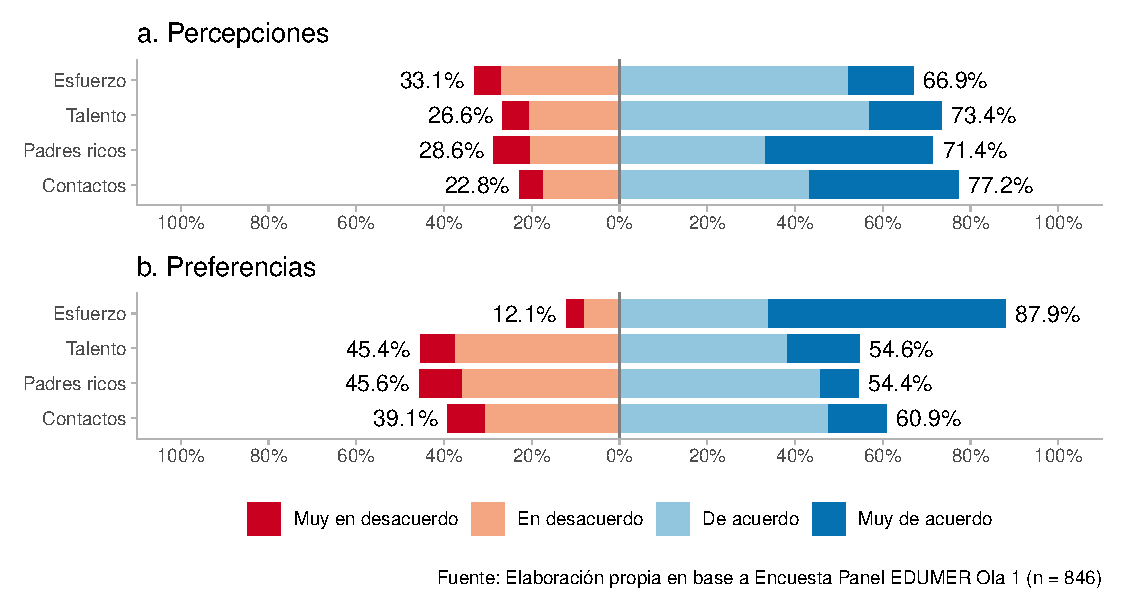
\includegraphics{entrega2_files/figure-pdf/fig-likert-1.pdf}

}

\end{figure}%

En la Table~\ref{tbl-correlaciones} se presenta la matriz de
correlaciones para los items de la escala. En términos generales, se
observa una correlación positiva y de magnitud moderada entre los ítems
que conforman una misma dimensión de la escala. Es decir, los ítems que
miden percepción de esfuerzo y talento (\(r\) = 0.52,
\(p\)\textless.05), así como los que miden percepción sobre padres ricos
y contactos (\(r\) = 0.61, \(p\)\textless.05), tienden a correlacionarse
entre sí. Este patrón también se reproduce en el caso de las
preferencias normativas, donde los ítems dentro de cada subdimensión
presentan correlaciones consistentes entre ellos.

No obstante, un hallazgo relevante es la presencia de correlaciones
positivas, aunque de magnitud débil a moderada, entre ítems que
pertenecen a dimensiones conceptualmente opuestas. Por ejemplo, se
observa que la percepción sobre la influencia de los padres ricos---un
elemento típicamente considerado no meritocrático---se asocia
positivamente con la preferencia por el esfuerzo---un criterio
meritocrático (\(r\) = 0.21). Este mismo patrón se observa con la
percepción sobre el uso de contactos, que también presenta una
correlación positiva con la preferencia por el esfuerzo (\(r\) = 0.26).

\begin{longtable}[]{@{}
  >{\raggedright\arraybackslash}p{(\columnwidth - 16\tabcolsep) * \real{0.3836}}
  >{\raggedright\arraybackslash}p{(\columnwidth - 16\tabcolsep) * \real{0.0959}}
  >{\raggedright\arraybackslash}p{(\columnwidth - 16\tabcolsep) * \real{0.0959}}
  >{\raggedright\arraybackslash}p{(\columnwidth - 16\tabcolsep) * \real{0.0822}}
  >{\raggedright\arraybackslash}p{(\columnwidth - 16\tabcolsep) * \real{0.0685}}
  >{\raggedright\arraybackslash}p{(\columnwidth - 16\tabcolsep) * \real{0.0822}}
  >{\raggedright\arraybackslash}p{(\columnwidth - 16\tabcolsep) * \real{0.0685}}
  >{\raggedright\arraybackslash}p{(\columnwidth - 16\tabcolsep) * \real{0.0685}}
  >{\raggedright\arraybackslash}p{(\columnwidth - 16\tabcolsep) * \real{0.0548}}@{}}

\caption{\label{tbl-correlaciones}Matriz de correlaciones policóricas
entre los ítems de Escala de Meritocracia}

\tabularnewline

\toprule\noalign{}
\begin{minipage}[b]{\linewidth}\raggedright
\end{minipage} & \begin{minipage}[b]{\linewidth}\raggedright
(A)
\end{minipage} & \begin{minipage}[b]{\linewidth}\raggedright
(B)
\end{minipage} & \begin{minipage}[b]{\linewidth}\raggedright
(C)
\end{minipage} & \begin{minipage}[b]{\linewidth}\raggedright
(D)
\end{minipage} & \begin{minipage}[b]{\linewidth}\raggedright
(E)
\end{minipage} & \begin{minipage}[b]{\linewidth}\raggedright
(F)
\end{minipage} & \begin{minipage}[b]{\linewidth}\raggedright
(G)
\end{minipage} & \begin{minipage}[b]{\linewidth}\raggedright
(H)
\end{minipage} \\
\midrule\noalign{}
\endhead
\bottomrule\noalign{}
\endlastfoot
A. Percepción Esfuerzo & & & & & & & & \\
B. Percepción Talento & 0.52* & & & & & & & \\
C. Percepción Padres Ricos & -0.16 & -0.04. & & & & & & \\
D. Percepción Contactos & -0.10* & 0.01* & 0.61* & & & & & \\
E. Preferencia Esfuerzo & 0.01 & 0.12 & 0.21 & 0.26 & & & & \\
F. Preferencia Talento & -0.04 & 0.08 & 0.16 & 0.25 & 0.36* & & & \\
G. Preferencia Padres Ricos & 0.06 & 0.10 & 0.15 & 0.19 & 0.05 & 0.10 &
& \\
H. Preferencia Contactos & 0.11 & 0.09 & 0.06 & 0.26 & 0.06 & 0.12 &
0.61 & \\

\end{longtable}

\textbf{Note:} **p\textless0.01, *p\textless0.5

\subsection{Multivariados}\label{multivariados}

\subsubsection{Análisis factorial
confirmatorio}\label{anuxe1lisis-factorial-confirmatorio}

En la Figure~\ref{fig-cfa1} se presenta la solución estandarizada del
modelo factorial confirmatorio estimado para la escala de meritocracia
en la primera ola del estudio. De acuerdo con los grados de libertad, el
modelo se encuentra sobre identidicado (\(df\) = 14 \textgreater{} 0).
Los indicadores de ajuste global muestran que el modelo presenta un buen
ajuste a los datos empíricos. En efecto, tanto el índice de ajuste
comparativo (CFI) como el índice de Tucker-Lewis (TLI) y el error
cuadrático medio de aproximación (RMSEA) se encuentran dentro de los
umbrales comúnmente aceptados para indicar un buen ajuste (CFI y TLI
\textgreater{} 0.95; RMSEA \textless{} 0.05), lo cual respalda la
validez factorial del instrumento
(\citeproc{ref-brown_confirmatory_2015}{Brown, 2015}).

\begin{figure}

\caption{\label{fig-cfa1}Análisis factorial confirmatorio de Escala de
Meritocracia Ola 1}

\centering{

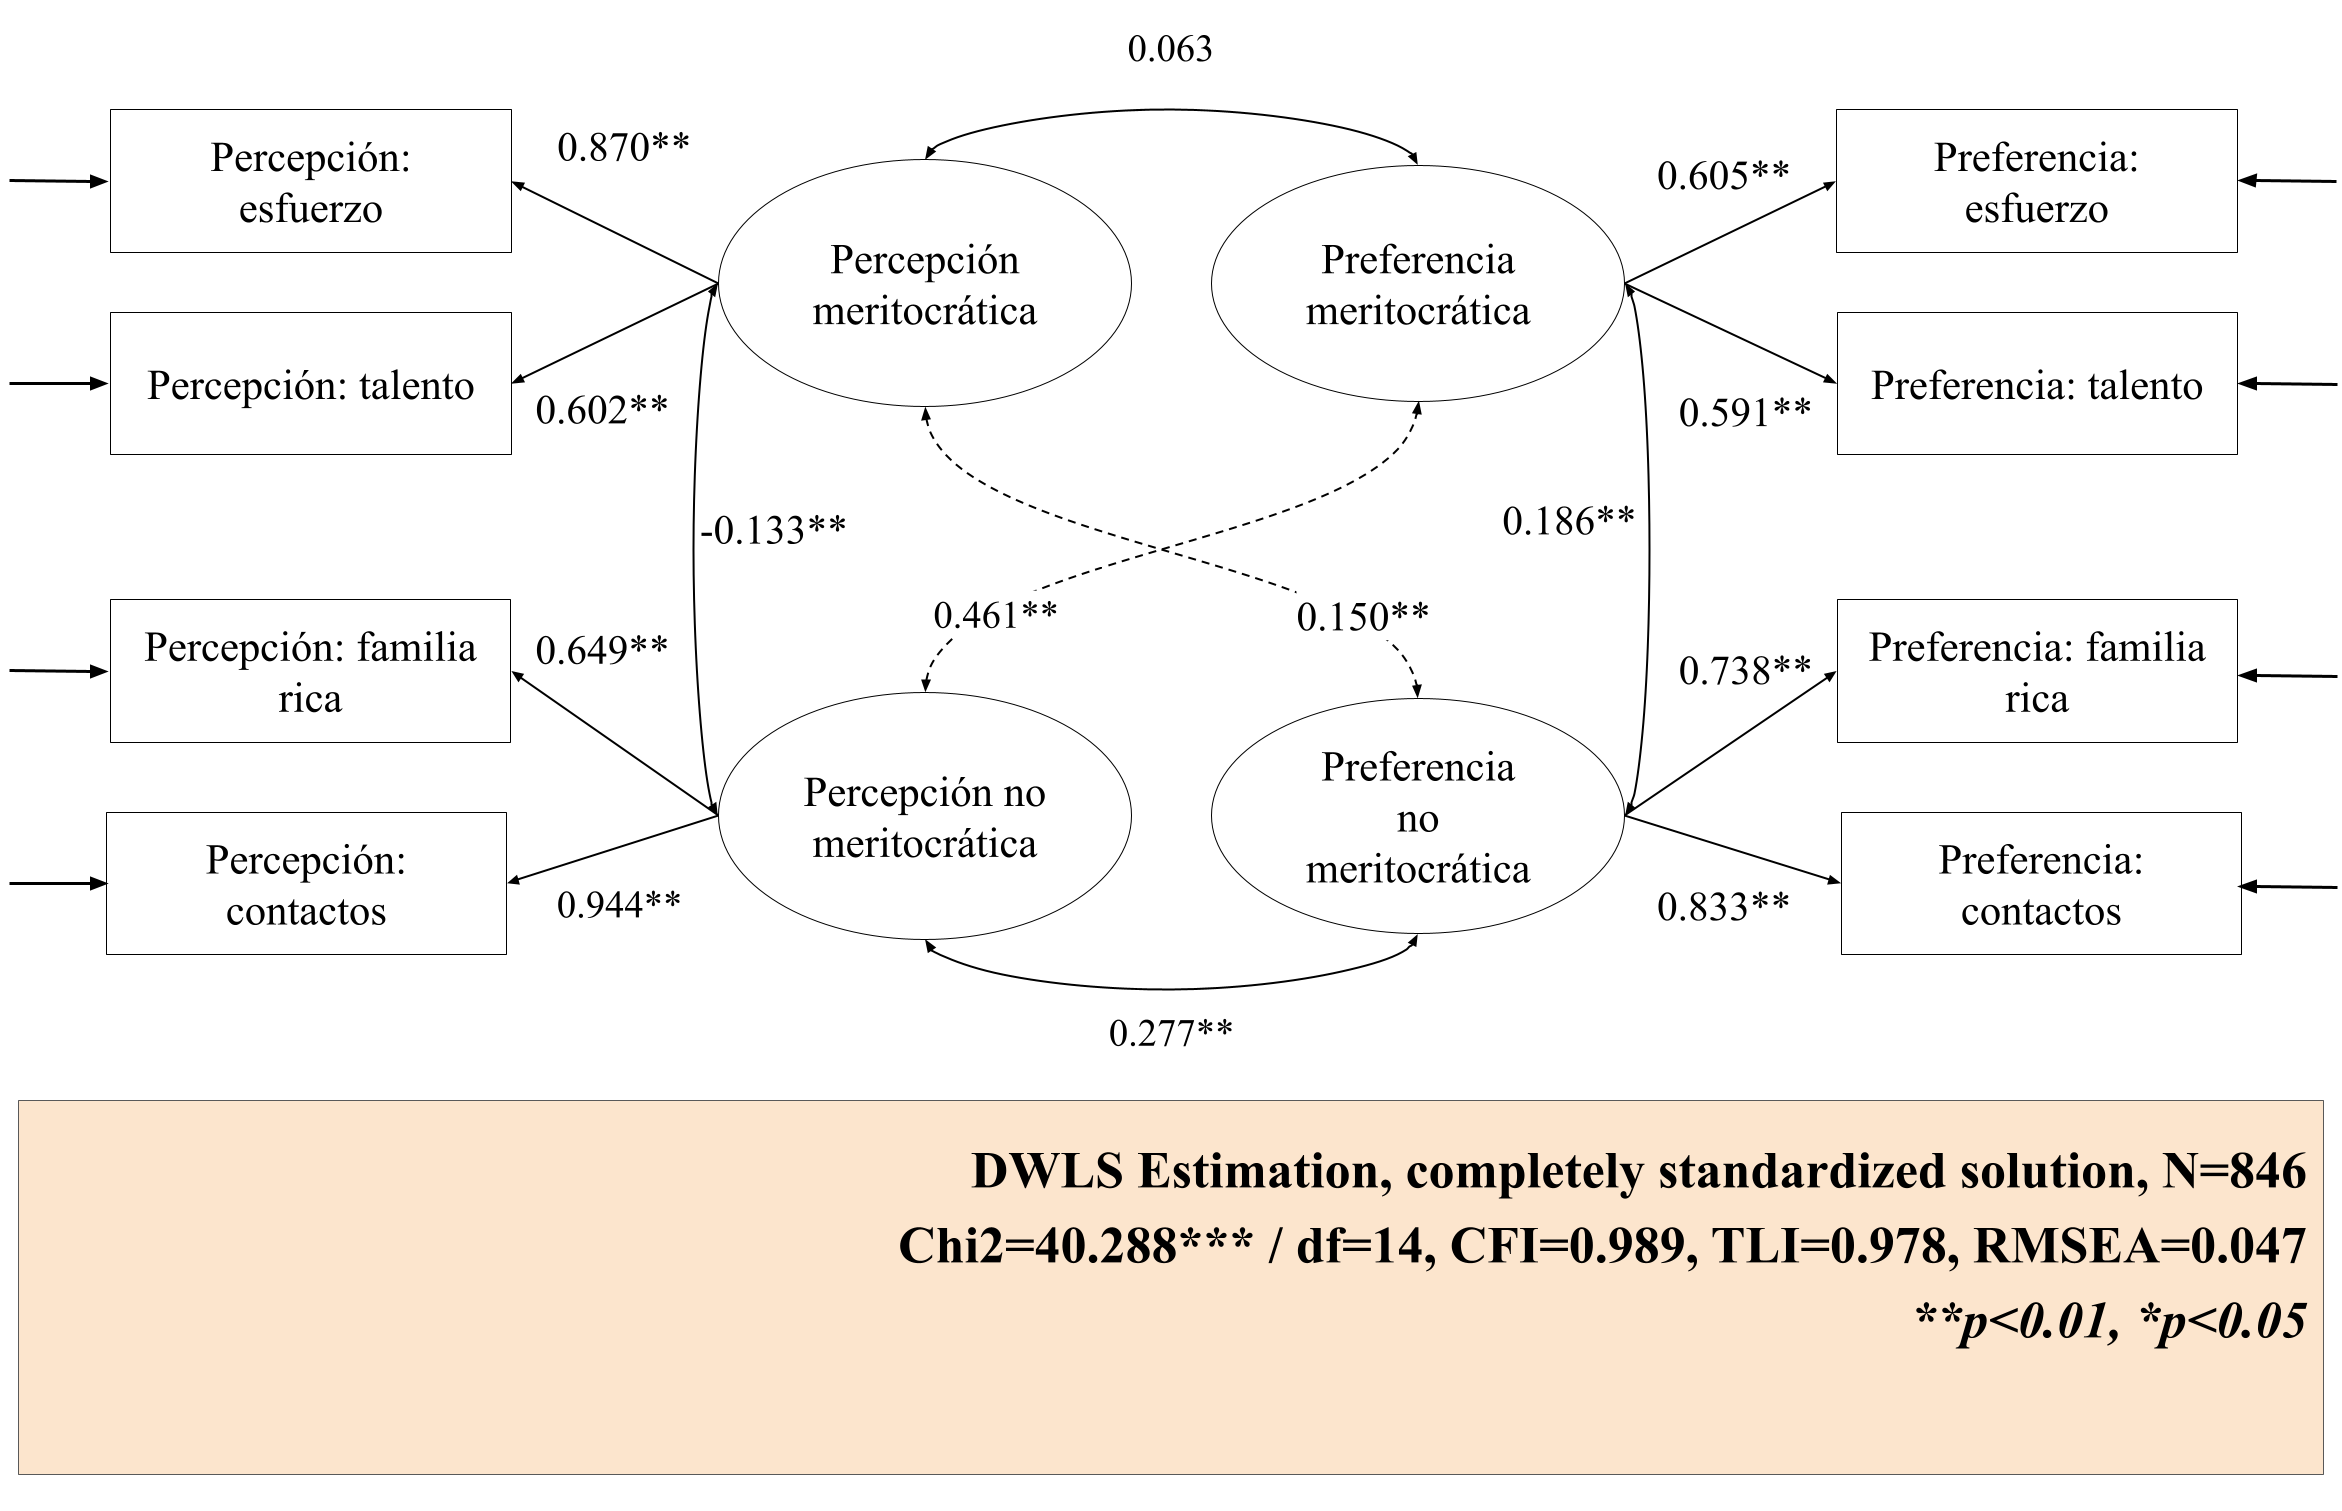
\includegraphics[width=1\textwidth,height=\textheight]{cfa_w1.png}

}

\end{figure}%

En relación con las cargas factoriales, todos los ítems se asocian de
forma positiva y estadísticamente significativa con sus respectivas
dimensiones latentes, y presentan cargas estandarizadas superiores a
0.5, lo que indica una adecuada calidad de la medición
(\citeproc{ref-brown_confirmatory_2015}{Brown, 2015}). Dentro de la
dimensión de percepción meritocrática, el ítem correspondiente al
esfuerzo destaca como el indicador con mayor carga factorial (\(\beta\)
= 0.87, \(p\) \textless{} 0.01), lo que sugiere que este principio
constituye el eje central en las creencias sobre los mecanismos
legítimos del éxito social desde una lógica meritocrática. Por su parte,
en la dimensión de percepción no meritocrática, el ítem referido al uso
de contactos personales presenta la mayor carga (\(\beta\) = 0.944,
\(p\) \textless{} 0.01), posicionándose como el componente más
representativo de esta dimensión. En las dimensiones normativas se
observan patrones similares: en la preferencia por criterios
meritocráticos existe una cierta paridad entre los ítems de esfuerzo y
talento, sin que uno predomine claramente sobre el otro, mientras que en
la preferencia por criterios no meritocráticos nuevamente el uso de
contactos (\(\beta\) = 0.833, \(p\) \textless{} 0.01) emerge como el
criterio normativo más relevante.

Respecto de las correlaciones entre factores, se identifican relaciones
conceptualmente significativas. Por un lado, la percepción de que los
logros sociales se deben a factores meritocráticos se asocia
negativamente con la percepción de que estos se explican por mecanismos
no meritocráticos (\(r\) = -0.133, \(p\)\textless0.01). Por otro lado, y
en contraste con esta lógica excluyente en el plano perceptivo, se
observa una correlación positiva entre las preferencias meritocráticas y
no meritocráticas (\(r\) = 0.186, \(p\)\textless0.01). Este hallazgo
sugiere que, normativamente, ambas lógicas pueden coexistir: los
estudiantes pueden simultáneamente valorar que el esfuerzo o el talento
deban ser recompensados, al mismo tiempo que consideran legítimo que
otros factores, como el origen familiar o los contactos, también
influyan en el acceso a ventajas.

Se observa una correlación positiva entre la percepción de mecanismos no
meritocráticos y la preferencia por mecanismos meritocráticos.
Específicamente, quienes perciben que el funcionamiento social se basa
en factores no meritocráticos ---como los contactos personales o el
origen familiar--- tienden a manifestar una mayor preferencia por que
elementos meritocráticos, como el esfuerzo y el talento, sean
efectivamente recompensados en la sociedad (\(r\) = 0.461, \(p\)
\textless{} 0.01). Este hallazgo sugiere que el reconocimiento de una
realidad social percibida como injusta o alejada del ideal meritocrático
puede reforzar normativamente la adhesión a principios meritocráticos.
En otras palabras, cuanto más se percibe que operan criterios ajenos al
mérito en la distribución de ventajas, mayor es el deseo de que el
mérito ---en particular, el esfuerzo y el talento--- se convierta en el
fundamento legítimo de la recompensa social.

\begin{figure}

\caption{\label{fig-cfa2}Análisis factorial confirmatorio de Escala de
Meritocracia Ola 2}

\centering{

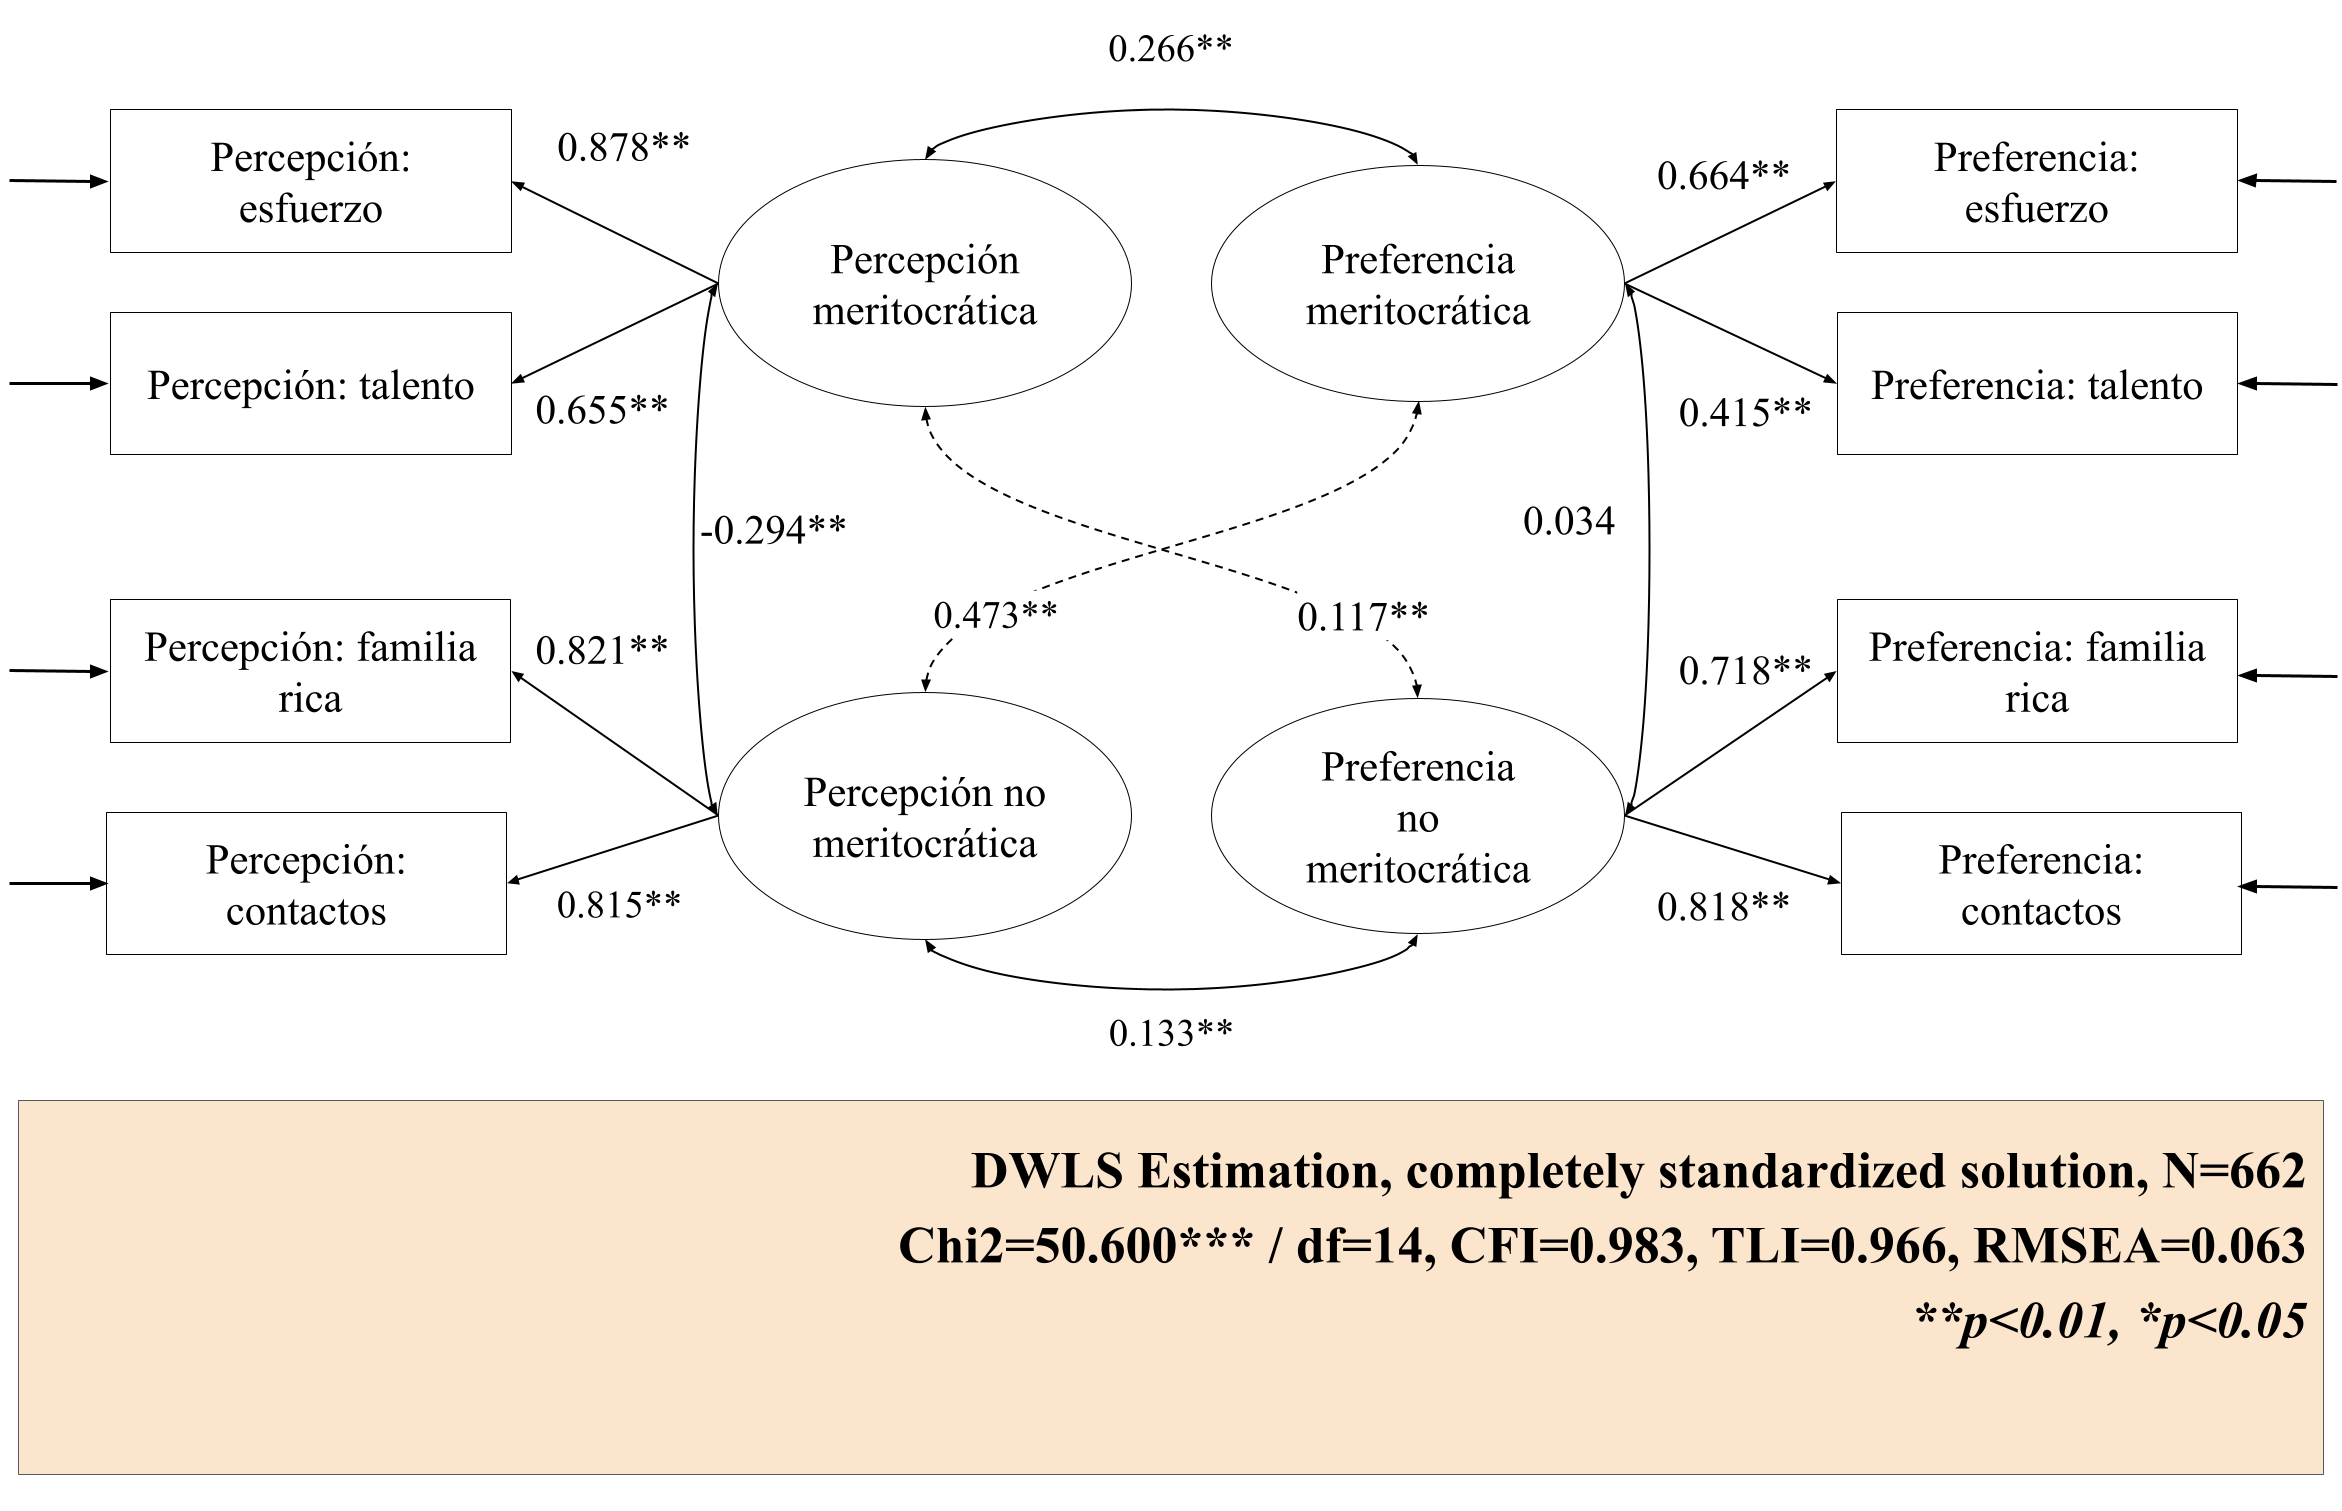
\includegraphics[width=1\textwidth,height=\textheight]{cfa_w2.png}

}

\end{figure}%

En la Figure~\ref{fig-cfa2} se presenta la solución estandarizada del
modelo factorial confirmatorio estimado para la segunda ola del estudio.
Al igual que en la ola anterior, el modelo se encuentra
sobreidentificado, con 14 grados de libertad (\(df\) = 14 \textgreater{}
0), lo que permite una estimación robusta de los parámetros del modelo.

En términos de ajuste global, los indicadores complementarios ---el
índice de ajuste comparativo (CFI) y el índice de Tucker-Lewis (TLI)---
se sitúan por sobre el umbral de 0.95, lo que indica un buen ajuste
relativo del modelo. Por su parte, el RMSEA alcanza un valor de 0.06,
que corresponde a un ajuste razonable según los criterios establecidos
en la literatura especializada
(\citeproc{ref-brown_confirmatory_2015}{Brown, 2015}).

En cuanto a las cargas factoriales, se mantienen los patrones observados
en la ola anterior con algunas variaciones menores. Dentro de la
dimensión de percepción meritocrática, el ítem de esfuerzo continúa
siendo el más relevante, mostrando una carga superior a la del talento.
En la percepción no meritocrática, en cambio, se observa una mayor
paridad entre los indicadores: tanto el ítem de padres ricos como el de
contactos personales contribuyen de manera similar a la dimensión. En lo
que respecta a las preferencias normativas, se confirma nuevamente que
el esfuerzo es el componente con mayor carga factorial dentro de la
dimensión meritocrática, superando al talento. Por su parte, en la
preferencia por criterios no meritocráticos, el ítem que presenta mayor
peso es el de contactos, reafirmando su centralidad en esta dimensión.

Respecto de las correlaciones entre factores, se replican en gran medida
los patrones observados en la primera ola. Se mantiene la correlación
negativa entre percepción meritocrática y percepción no meritocrática,
así como la correlación positiva entre las preferencias por criterios
meritocráticos y no meritocráticos, indicando la persistencia de una
tensión entre representación descriptiva y posicionamiento normativo.
También se conserva la asociación positiva entre percepción no
meritocrática y preferencia por estos mecanismos, lo que refuerza la
hipótesis de legitimación normativa de estructuras no basadas en mérito.

\subsubsection{Invarianza longitudinal}\label{invarianza-longitudinal}

Para evaluar la estabilidad estructural de la escala a lo largo del
tiempo, se estimaron modelos jerárquicos de invarianza longitudinal
utilizando análisis factorial confirmatorio (CFA) con indicadores
categóricos ordenados. En línea con las recomendaciones metodológicas de
Liu et al. (\citeproc{ref-liu_testing_2017}{2017}), se evaluaron cuatro
modelos anidados con estimación mediante mínimos cuadrados ponderados
diagonales con corrección robusta (WLSMV) y parametrización tipo theta.
Los modelos probados fueron: configural (estructura factorial libre),
débil (cargas factoriales iguales), fuerte (cargas y umbrales iguales),
y estricto (cargas, umbrales y varianzas residuales iguales).

El modelo especificado contempla cuatro factores latentes replicados en
dos mediciones (olas), cada uno con dos ítems. Se permitió la covarianza
de los errores de medición del mismo ítem entre las dos olas, una
práctica recomendada para modelos longitudinales con pocos indicadores
por factor. La identificación se logró fijando una carga a 1 por cada
factor y un umbral igualado por ítem entre olas.

\begingroup\fontsize{9}{11}\selectfont

\begin{longtable}[t]{cccccccc}

\caption{\label{tbl-invarianza}Pruebas de invarianza longitudinal para
el modelo de cuatro factores con indicadores ordinales}

\tabularnewline

\toprule
Model & \&chi;\textasciicircum{}2 (df) & CFI & RMSEA (90 CI) & \&Delta; \&chi;\textasciicircum{}2 (\&Delta; df) & \&Delta; CFI & \&Delta; RMSEA & Decision\\
\midrule
Configural & 117.7 (68) & 0.991 & 0.035 
 (0.024-0.046) & |            0 (0) & |      0 & |     0.000 & | Reference\\
Weak & 122.51 (72) & 0.990 & 0.034 
 (0.024-0.045) & |          4.809 (4) & |      0 & |    -0.001 & |  Accept\\
Strong & 128.53 (80) & 0.991 & 0.032 
 (0.021-0.042) & |           6.02 (8) & |      0 & |    -0.002 & |  Accept\\
Strict & 130.17 (84) & 0.991 & 0.031 
 (0.02-0.04) & |          1.635 (4) & |      0 & |    -0.002 & |  Accept\\
\bottomrule

\end{longtable}

\endgroup{}

En la Table~\ref{tbl-invarianza} se presentan los índices de ajuste
global para cada modelo, junto con las diferencias relativas entre
modelos consecutivos. Los valores de CFI ≥ 0.990 y RMSEA ≤ 0.035 en
todos los modelos sugieren un ajuste adecuado. Además, los cambios entre
modelos anidados fueron sistemáticamente inferiores a los puntos de
corte recomendados para evaluar deterioro del ajuste (\(\Delta\)CFI
\textless{} 0.01; \(\Delta\)RMSEA \textless{} 0.015), lo que respalda la
aceptación de los supuestos de invarianza en cada nivel.

En conjunto, estos resultados respaldan la existencia de invarianza
estricta longitudinal, lo que permite comparar de manera válida las
puntuaciones latentes entre las dos olas del estudio. Esto implica que
los cambios observados pueden atribuirse a diferencias reales en las
percepciones y preferencias meritocráticas de los estudiantes, y no a
cambios en la interpretación o funcionamiento de los ítems a lo largo
del tiempo.

\section{Referencias}\label{referencias}

\phantomsection\label{refs}
\begin{CSLReferences}{1}{0}
\bibitem[\citeproctext]{ref-batruch_belief_2022}
Batruch, A., Jetten, J., Van de Werfhorst, H., Darnon, C., \& Butera, F.
(2022). Belief in {School Meritocracy} and the {Legitimization} of
{Social} and {Income Inequality}. \emph{Social Psychological and
Personality Science}, 194855062211110.
\url{https://doi.org/10.1177/19485506221111017}

\bibitem[\citeproctext]{ref-brown_confirmatory_2015}
Brown, T. A. (2015). \emph{Confirmatory factor analysis for applied
research} (Second edition). New York London: The Guilford Press.

\bibitem[\citeproctext]{ref-castillo_multidimensional_2023}
Castillo, J. C., Iturra, J., Maldonado, L., Atria, J., \& Meneses, F.
(2023). A {Multidimensional Approach} for {Measuring Meritocratic
Beliefs}: {Advantages}, {Limitations} and {Alternatives} to the {ISSP
Social Inequality Survey}. \emph{International Journal of Sociology},
\emph{53}(6), 448--472.
\url{https://doi.org/10.1080/00207659.2023.2274712}

\bibitem[\citeproctext]{ref-chancel_world_2022}
Chancel, L., Piketty, T., Saez, E., \& Zucman, G. (2022). World
inequality report 2022.
https://bibliotecadigital.ccb.org.co/handle/11520/27510.

\bibitem[\citeproctext]{ref-chen_sensitivity_2007}
Chen, F. F. (2007). Sensitivity of {Goodness} of {Fit Indexes} to {Lack}
of {Measurement Invariance}. \emph{Structural Equation Modeling: A
Multidisciplinary Journal}, \emph{14}(3), 464--504.
\url{https://doi.org/10.1080/10705510701301834}

\bibitem[\citeproctext]{ref-corvalan_mercado_2017}
Corvalán, J., Carrasco, A., \& García-Huidobro;J. E. (2017).
\emph{Mercado escolar: {Libertad}, diversidad y desigualdad}. Ediciones
UC.

\bibitem[\citeproctext]{ref-darnon_where_2018}
Darnon, C., Wiederkehr, V., Dompnier, B., \& Martinot, D. (2018).
{``{Where} there is a will, there is a way''}: {Belief} in school
meritocracy and the social-class achievement gap. \emph{British Journal
of Social Psychology}, \emph{57}(1), 250--262.
\url{https://doi.org/10.1111/bjso.12214}

\bibitem[\citeproctext]{ref-davidov_measurement_2014}
Davidov, E., Meuleman, B., Cieciuch, J., Schmidt, P., \& Billiet, J.
(2014). Measurement {Equivalence} in {Cross-National Research}.
\emph{Annual Review of Sociology}, \emph{40}(Volume 40, 2014), 55--75.
\url{https://doi.org/10.1146/annurev-soc-071913-043137}

\bibitem[\citeproctext]{ref-dubet_repensar_2011}
Dubet, F. (2011). \emph{{Repensar la justicia social}} (Sexta
Edici{ó}n). Siglo XXI.

\bibitem[\citeproctext]{ref-kline_principles_2023}
Kline, R. B. (2023). \emph{Principles and {Practice} of {Structural
Equation Modeling}}. Guilford Publications.

\bibitem[\citeproctext]{ref-liu_testing_2017}
Liu, Y., Millsap, R. E., West, S. G., Tein, J.-Y., Tanaka, R., \& Grimm,
K. J. (2017). Testing measurement invariance in longitudinal data with
ordered-categorical measures. \emph{Psychological Methods},
\emph{22}(3), 486--506. \url{https://doi.org/10.1037/met0000075}

\bibitem[\citeproctext]{ref-mijs_paradox_2019}
Mijs, J. (2019). The paradox of inequality: Income inequality and belief
in meritocracy go hand in hand. \emph{Socio-Economic Review},
\emph{19}(1), 7--35. \url{https://doi.org/10.1093/ser/mwy051}

\bibitem[\citeproctext]{ref-wiederkehr_belief_2015}
Wiederkehr, V., Bonnot, V., Krauth-Gruber, S., \& Darnon, C. (2015).
Belief in school meritocracy as a system-justifying tool for low status
students. \emph{Frontiers in Psychology}, \emph{6}.

\bibitem[\citeproctext]{ref-wilson_role_2003a}
Wilson, C. (2003). The {Role} of a {Merit Principle} in {Distributive
Justice}. \emph{The Journal of Ethics}, \emph{7}(3), 277--314.
\url{https://doi.org/10.1023/A:1024667228488}

\bibitem[\citeproctext]{ref-young_rise_1958}
Young, M. (1958). \emph{The rise of the meritocracy}. New Brunswick,
N.J., U.S.A: Transaction Publishers.

\end{CSLReferences}

\pagebreak

\section{Anexos}\label{anexos}

\subsection{Análisis factorial
exploratorio}\label{anuxe1lisis-factorial-exploratorio}

\begin{Shaded}
\begin{Highlighting}[]
 \FunctionTok{tab\_fa}\NormalTok{(db\_w1, }\AttributeTok{method =} \StringTok{"ml"}\NormalTok{, }\AttributeTok{rotation =} \StringTok{"varimax"}\NormalTok{, }\AttributeTok{show.comm =} \ConstantTok{TRUE}\NormalTok{)}
\end{Highlighting}
\end{Shaded}

\begin{verbatim}
Parallel analysis suggests that the number of factors =  4  and the number of components =  NA 
\end{verbatim}

\begin{longtable}[]{@{}
  >{\raggedright\arraybackslash}p{(\columnwidth - 10\tabcolsep) * \real{0.1667}}
  >{\raggedright\arraybackslash}p{(\columnwidth - 10\tabcolsep) * \real{0.1667}}
  >{\raggedright\arraybackslash}p{(\columnwidth - 10\tabcolsep) * \real{0.1667}}
  >{\raggedright\arraybackslash}p{(\columnwidth - 10\tabcolsep) * \real{0.1667}}
  >{\raggedright\arraybackslash}p{(\columnwidth - 10\tabcolsep) * \real{0.1667}}
  >{\raggedright\arraybackslash}p{(\columnwidth - 10\tabcolsep) * \real{0.1667}}@{}}

\caption{\label{tbl-exploratorio}Análisis exploratorio escala de
meritocracia}

\tabularnewline

\caption{Factor Analysis}\tabularnewline
\toprule\noalign{}
\endfirsthead
\endhead
\bottomrule\noalign{}
\endlastfoot
~ & Factor 1 & Factor 2 & Factor 3 & Factor 4 & Communality \\
\begin{minipage}[t]{\linewidth}\raggedright
En Chile, las personas son recompensadas\\
por sus esfuerzos\strut
\end{minipage} & 0.07 & -0.09 & 0.59 & -0.04 & 0.36 \\
\begin{minipage}[t]{\linewidth}\raggedright
En Chile, las personas son recompensadas\\
por su inteligencia y habilidad\strut
\end{minipage} & 0.04 & 0.02 & 0.76 & 0.12 & 0.60 \\
\begin{minipage}[t]{\linewidth}\raggedright
En Chile, a quienes tienen padres ricos\\
les va mucho mejor en la vida\strut
\end{minipage} & 0.04 & 0.99 & -0.07 & 0.12 & 0.99 \\
\begin{minipage}[t]{\linewidth}\raggedright
En Chile, quienes tienen buenos\\
contactos les va mejor en la vida\strut
\end{minipage} & 0.20 & 0.49 & -0.04 & 0.30 & 0.37 \\
\begin{minipage}[t]{\linewidth}\raggedright
Quienes más se esfuerzan deberían\\
obtener mayores recompensas que quienes\\
se esfuerzan menos\strut
\end{minipage} & 0.01 & 0.12 & 0.06 & 0.47 & 0.24 \\
\begin{minipage}[t]{\linewidth}\raggedright
Quienes poseen más talento deberían\\
obtener mayores recompensas que quienes\\
poseen menos talento\strut
\end{minipage} & 0.07 & 0.07 & -0.01 & 0.57 & 0.33 \\
\begin{minipage}[t]{\linewidth}\raggedright
Está bien que quienes tienen padres\\
ricos les vaya bien en la vida\strut
\end{minipage} & 0.53 & 0.12 & 0.07 & 0.05 & 0.31 \\
\begin{minipage}[t]{\linewidth}\raggedright
Está bien que quienes tienen buenos\\
contactos les vaya bien en la vida\strut
\end{minipage} & 0.99 & 0.01 & 0.05 & 0.07 & 0.99 \\
Total Communalities &
\multicolumn{4}{>{\centering\arraybackslash}p{(\columnwidth - 10\tabcolsep) * \real{0.6667} + 6\tabcolsep}}{%
} & 4.19 \\
Cronbach\textquotesingle s α & 0.70 & 0.69 & 0.61 & 0.43 & \\

\end{longtable}

Como primera parte del análisis, se aplicó la adecuación muestral (KMO),
dando como resultado correlaciones de magnitud moderada de manera
generalizada (Ver anexos). Esto quiere decir que los resultados son
adecuados para realizar un Análisis Factorial Exploratorio. Además se
aplicó un test de esfericidad de Bartlett el cual dio significancia
estadística, por lo que se puede afirmar que la matriz de correlaciones
observada es una matriz identidad (\(p\)\textless.05).

En la Table~\ref{tbl-exploratorio} se pueden observar los resultados del
análisis factorial exploratorio realizado a partir del método Maximum
likelihood con una rotación ortogonal. Se puede observar la presencia de
cuatro factores, pero resultan llamativos los factores 1 y 2,
específicamente las cargas factoriales de preferencia de contactos y la
percepción de padres ricos, respectivamente. Ambos indicadores tienen
una carga factorial de 0.99 y una comunalidad del mismo valor. Su
interpretación sugiere que ambos indicadores se asocian casi por
completo a un factor, por lo que el indicador con menor carga factorial
en los factores 1 y 2 podría ser prescindido. No obstante, este
resultado que debe tomarse con precaución, puesto que el método para la
extracción de factores empleado fue ML, el cual tiende a maximizar la
probabilidad de que los parámetros reproduzcan los parámetros
observados, por lo que podría haber generado algún tipo de sobreajuste.

Por otro lado, al aplicar el método de Ejes Principales, las cargas
factoriales de 0.99 que se generaban en el caso anterior disminuyen,
pero aún así mantienen una alta comunalidad. Es importante mencionar que
todos los indicadores poseen una complejidad \textgreater{} 1, lo cual
señala que cada ítem representa un único constructo subyacente. Por
último, la suma de cargas al cuadrado para los dos primeros factores el
\textgreater{} 1, por lo que son factores que vale la pena conservar. En
cambio, los factores 3 y 4 poseen valores \textless{} 1 (0.913 y 0.631,
respectivamente), lo cual resulta problemático para la escala analizada.
Si bien, en términos de conveniencia estadística sería mejor eliminar el
factor 4 de la escala, esto no puede realizarse debido a la relevancia
teórica que posee para el instrumento de medición, por ello es
importante tomar en consideración este resultado para posteriores usos.

\begin{Shaded}
\begin{Highlighting}[]
\FunctionTok{KMO}\NormalTok{(corMat) }
\end{Highlighting}
\end{Shaded}

\begin{verbatim}
Kaiser-Meyer-Olkin factor adequacy
Call: KMO(r = corMat)
Overall MSA =  0.56
MSA for each item = 
      perc_effort       perc_talent perc_rich_parents      perc_contact 
             0.52              0.52              0.55              0.59 
      pref_effort       pref_talent pref_rich_parents      pref_contact 
             0.67              0.67              0.55              0.52 
\end{verbatim}

\begin{Shaded}
\begin{Highlighting}[]
\FunctionTok{cortest.bartlett}\NormalTok{(corMat, }\AttributeTok{n =} \DecValTok{846}\NormalTok{)}
\end{Highlighting}
\end{Shaded}

\begin{verbatim}
$chisq
[1] 986.5685

$p.value
[1] 0.0000000000000000000000000000000000000000000000000000000000000000000000000000000000000000000000000000000000000000000000000000000000000000000000000000000000000000000000000000000000000000000009929485

$df
[1] 28
\end{verbatim}

\begin{Shaded}
\begin{Highlighting}[]
\FunctionTok{scree.plot}\NormalTok{(db\_w1)}
\end{Highlighting}
\end{Shaded}

\begin{figure}[H]

\caption{\label{fig-scree}Gráfico de sedimentación}

\centering{

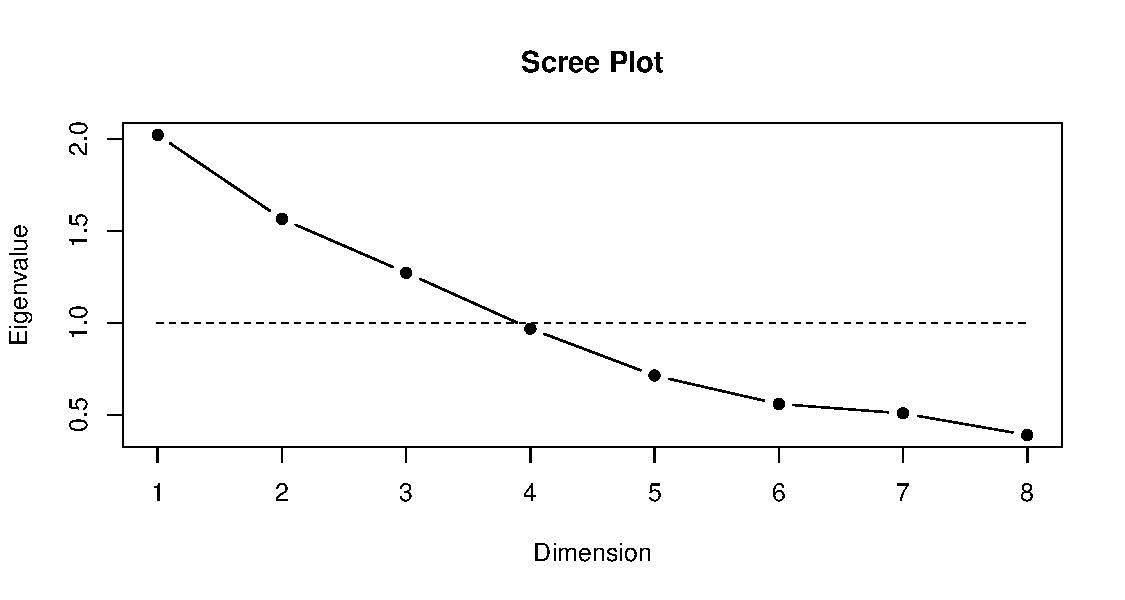
\includegraphics{entrega2_files/figure-pdf/fig-scree-1.pdf}

}

\end{figure}%

\begin{Shaded}
\begin{Highlighting}[]
\NormalTok{fac\_pa\_t}\OtherTok{\textless{}{-}}\FunctionTok{fa\_table}\NormalTok{(fac\_pa)}
\NormalTok{fac\_pa\_t}\SpecialCharTok{$}\NormalTok{ind\_table}
\end{Highlighting}
\end{Shaded}

\begin{table}
\caption*{
{\large Factor analysis results}
} 
\fontsize{12.0pt}{14.4pt}\selectfont
\begin{tabular*}{\linewidth}{@{\extracolsep{\fill}}l|rrrrrrr}
\toprule
 & Factor\_1 & Factor\_2 & Factor\_3 & Factor\_4 & Communality & Uniqueness & Complexity \\ 
\midrule\addlinespace[2.5pt]
pref\_contact & 0.919 & {\itshape \textcolor[HTML]{D3D3D3}{-0.024}} & {\itshape \textcolor[HTML]{D3D3D3}{-0.005}} & {\itshape \textcolor[HTML]{D3D3D3}{0.002}} & 0.84 & 0.16 & 1.00 \\ 
pref\_rich\_parents & 0.576 & {\itshape \textcolor[HTML]{D3D3D3}{0.096}} & {\itshape \textcolor[HTML]{D3D3D3}{0.035}} & {\itshape \textcolor[HTML]{D3D3D3}{-0.028}} & 0.36 & 0.64 & 1.07 \\ 
perc\_rich\_parents & {\itshape \textcolor[HTML]{D3D3D3}{-0.030}} & 0.868 & {\itshape \textcolor[HTML]{D3D3D3}{-0.005}} & {\itshape \textcolor[HTML]{D3D3D3}{-0.034}} & 0.73 & 0.27 & 1.01 \\ 
perc\_contact & {\itshape \textcolor[HTML]{D3D3D3}{0.134}} & 0.547 & {\itshape \textcolor[HTML]{D3D3D3}{-0.007}} & {\itshape \textcolor[HTML]{D3D3D3}{0.162}} & 0.44 & 0.56 & 1.30 \\ 
perc\_talent & {\itshape \textcolor[HTML]{D3D3D3}{-0.014}} & {\itshape \textcolor[HTML]{D3D3D3}{0.036}} & 0.672 & {\itshape \textcolor[HTML]{D3D3D3}{0.077}} & 0.46 & 0.54 & 1.03 \\ 
perc\_effort & {\itshape \textcolor[HTML]{D3D3D3}{0.021}} & {\itshape \textcolor[HTML]{D3D3D3}{-0.047}} & 0.670 & {\itshape \textcolor[HTML]{D3D3D3}{-0.075}} & 0.46 & 0.54 & 1.04 \\ 
pref\_talent & {\itshape \textcolor[HTML]{D3D3D3}{0.015}} & {\itshape \textcolor[HTML]{D3D3D3}{-0.027}} & {\itshape \textcolor[HTML]{D3D3D3}{-0.028}} & 0.590 & 0.34 & 0.66 & 1.01 \\ 
pref\_effort & {\itshape \textcolor[HTML]{D3D3D3}{-0.058}} & {\itshape \textcolor[HTML]{D3D3D3}{0.060}} & {\itshape \textcolor[HTML]{D3D3D3}{0.072}} & 0.466 & 0.24 & 0.76 & 1.11 \\ 
\bottomrule
\end{tabular*}
\end{table}

\begin{Shaded}
\begin{Highlighting}[]
\NormalTok{fac\_pa\_t}\SpecialCharTok{$}\NormalTok{f\_table}
\end{Highlighting}
\end{Shaded}

\begin{table}
\caption*{
{\large Eigenvalues, Variance Explained, and Factor Correlations for Rotated Factor Solution}
} 
\fontsize{12.0pt}{14.4pt}\selectfont
\begin{tabular*}{\linewidth}{@{\extracolsep{\fill}}lrrrr}
\toprule
Property & Factor\_1 & Factor\_2 & Factor\_3 & Factor\_4 \\ 
\midrule\addlinespace[2.5pt]
SS loadings & 1.209 & 1.108 & 0.913 & 0.631 \\ 
Proportion Var & 0.151 & 0.138 & 0.114 & 0.079 \\ 
Cumulative Var & 0.151 & 0.290 & 0.404 & 0.483 \\ 
Proportion Explained & 0.313 & 0.287 & 0.236 & 0.163 \\ 
Cumulative Proportion & 0.313 & 0.600 & 0.837 & 1.000 \\ 
Factor\_1 & 1.000 & 0.146 & 0.144 & 0.196 \\ 
Factor\_2 & 0.146 & 1.000 & -0.111 & 0.364 \\ 
Factor\_3 & 0.144 & -0.111 & 1.000 & 0.072 \\ 
Factor\_4 & 0.196 & 0.364 & 0.072 & 1.000 \\ 
\bottomrule
\end{tabular*}
\end{table}

\section{Código de R}\label{cuxf3digo-de-r}

\begin{Shaded}
\begin{Highlighting}[]
\FunctionTok{library}\NormalTok{(knitr)}
\NormalTok{knitr}\SpecialCharTok{::}\NormalTok{opts\_chunk}\SpecialCharTok{$}\FunctionTok{set}\NormalTok{(}\AttributeTok{echo =} \ConstantTok{TRUE}\NormalTok{, }\AttributeTok{include =} \ConstantTok{TRUE}\NormalTok{, }\AttributeTok{warning =} \ConstantTok{FALSE}\NormalTok{, }\AttributeTok{message =} \ConstantTok{FALSE}\NormalTok{)}

\NormalTok{table\_format }\OtherTok{\textless{}{-}} \ControlFlowTok{if}\NormalTok{(}\FunctionTok{is\_html\_output}\NormalTok{()) \{}
  \StringTok{"html"}
\NormalTok{\} }\ControlFlowTok{else} \ControlFlowTok{if}\NormalTok{(}\FunctionTok{is\_latex\_output}\NormalTok{()) \{}
  \StringTok{"latex"}
\NormalTok{\}}
\NormalTok{table\_format2 }\OtherTok{\textless{}{-}} \ControlFlowTok{if}\NormalTok{(}\FunctionTok{is\_html\_output}\NormalTok{()) \{}
\NormalTok{  T}
\NormalTok{\} }\ControlFlowTok{else} \ControlFlowTok{if}\NormalTok{(}\FunctionTok{is\_latex\_output}\NormalTok{()) \{}
\NormalTok{  F}
\NormalTok{\}}

\FunctionTok{options}\NormalTok{(}\AttributeTok{kableExtra.html.bsTable =}\NormalTok{ T)}
\FunctionTok{options}\NormalTok{(}\AttributeTok{knitr.kable.NA =} \StringTok{""}\NormalTok{)}
\ControlFlowTok{if}\NormalTok{ (}\SpecialCharTok{!} \FunctionTok{require}\NormalTok{(}\StringTok{"pacman"}\NormalTok{)) }\FunctionTok{install.packages}\NormalTok{(}\StringTok{"pacman"}\NormalTok{)}

\NormalTok{pacman}\SpecialCharTok{::}\FunctionTok{p\_load}\NormalTok{(tidyverse,}
\NormalTok{               sjmisc, }
\NormalTok{               sjPlot,}
\NormalTok{               here,}
\NormalTok{               lavaan,}
\NormalTok{               devtools,}
\NormalTok{               psych,}
\NormalTok{               psy,}
\NormalTok{               corrplot,}
\NormalTok{               ggdist,}
\NormalTok{               GPArotations,}
\NormalTok{               ggrepel,}
\NormalTok{               nfactors,}
\NormalTok{               patchwork,}
\NormalTok{               sjlabelled,}
\NormalTok{               semTools,}
\NormalTok{               gtools,}
\NormalTok{               RColorBrewer,}
\NormalTok{               skimr,}
\NormalTok{               readxl,}
\NormalTok{               tydiverse,}
\NormalTok{               kableExtra,}
\NormalTok{               xtable)}


\FunctionTok{options}\NormalTok{(}\AttributeTok{scipen=}\DecValTok{999}\NormalTok{)}
\FunctionTok{rm}\NormalTok{(}\AttributeTok{list =} \FunctionTok{ls}\NormalTok{())}
\FunctionTok{load}\NormalTok{(}\AttributeTok{file =} \FunctionTok{here}\NormalTok{(}\StringTok{"output"}\NormalTok{, }\StringTok{"data"}\NormalTok{, }\StringTok{"db\_long\_proc.RData"}\NormalTok{))}


\FunctionTok{names}\NormalTok{(db\_long)}
\FunctionTok{glimpse}\NormalTok{(db\_long)}

\NormalTok{tabla\_merit }\OtherTok{\textless{}{-}} \FunctionTok{data.frame}\NormalTok{(}
  \AttributeTok{Componente =} \FunctionTok{c}\NormalTok{(}\StringTok{"Percepción"}\NormalTok{, }\StringTok{""}\NormalTok{, }\StringTok{""}\NormalTok{, }\StringTok{""}\NormalTok{, }
                 \StringTok{"Preferencia"}\NormalTok{, }\StringTok{""}\NormalTok{, }\StringTok{""}\NormalTok{, }\StringTok{""}\NormalTok{),}
\NormalTok{  Dimensión }\OtherTok{=} \FunctionTok{c}\NormalTok{(}\StringTok{"Meritocrática"}\NormalTok{, }\StringTok{"Meritocrática"}\NormalTok{, }
                \StringTok{"No meritocrática"}\NormalTok{, }\StringTok{"No meritocrática"}\NormalTok{,}
                \StringTok{"Meritocrática"}\NormalTok{, }\StringTok{"Meritocrática"}\NormalTok{, }
                \StringTok{"No meritocrática"}\NormalTok{, }\StringTok{"No meritocrática"}\NormalTok{),}
\NormalTok{  Í}\AttributeTok{tem =} \FunctionTok{c}\NormalTok{(}
    \StringTok{"En Chile, las personas son recompensadas por su esfuerzo."}\NormalTok{,}
    \StringTok{"En Chile, las personas son recompensadas por su inteligencia y habilidades."}\NormalTok{,}
    \StringTok{"En Chile, a quienes tienen padres ricos les va mucho mejor en la vida."}\NormalTok{,}
    \StringTok{"En Chile, a quienes tienen buenos contactos les va mejor en la vida."}\NormalTok{,}
    \StringTok{"Quienes se esfuerzan más deberían recibir mayores recompensas que quienes se esfuerzan menos."}\NormalTok{,}
    \StringTok{"Quienes tienen más talento deberían recibir mayores recompensas que quienes tienen menos talento."}\NormalTok{,}
    \StringTok{"Está bien que a quienes tienen padres ricos les vaya bien en la vida."}\NormalTok{,}
    \StringTok{"Está bien que a quienes tienen buenos contactos les vaya bien en la vida."}
\NormalTok{  )}
\NormalTok{)}

\NormalTok{tabla\_merit }\SpecialCharTok{\%\textgreater{}\%}\NormalTok{ kableExtra}\SpecialCharTok{::}\FunctionTok{kable}\NormalTok{(., }\AttributeTok{format =} \StringTok{"markdown"}\NormalTok{)}

\FunctionTok{theme\_set}\NormalTok{(}\FunctionTok{theme\_ggdist}\NormalTok{())}
\NormalTok{colors }\OtherTok{\textless{}{-}}\NormalTok{ RColorBrewer}\SpecialCharTok{::}\FunctionTok{brewer.pal}\NormalTok{(}\AttributeTok{n =} \DecValTok{4}\NormalTok{, }\AttributeTok{name =} \StringTok{"RdBu"}\NormalTok{)}

\NormalTok{a }\OtherTok{\textless{}{-}}\NormalTok{ db\_long }\SpecialCharTok{\%\textgreater{}\%} 
  \FunctionTok{filter}\NormalTok{(ola }\SpecialCharTok{==} \DecValTok{1}\NormalTok{) }\SpecialCharTok{\%\textgreater{}\%}
  \FunctionTok{select}\NormalTok{(}\FunctionTok{starts\_with}\NormalTok{(}\StringTok{"perc"}\NormalTok{)) }\SpecialCharTok{\%\textgreater{}\%} 
\NormalTok{  sjPlot}\SpecialCharTok{::}\FunctionTok{plot\_likert}\NormalTok{(}\AttributeTok{geom.colors =}\NormalTok{ colors,}
                      \AttributeTok{title =} \FunctionTok{c}\NormalTok{(}\StringTok{"a. Percepciones"}\NormalTok{),}
                      \AttributeTok{geom.size =} \FloatTok{0.8}\NormalTok{,}
                      \AttributeTok{axis.labels =} \FunctionTok{c}\NormalTok{(}\StringTok{"Esfuerzo"}\NormalTok{, }\StringTok{"Talento"}\NormalTok{, }\StringTok{"Padres ricos"}\NormalTok{, }\StringTok{"Contactos"}\NormalTok{),}
                      \AttributeTok{catcount =} \DecValTok{4}\NormalTok{,}
                      \AttributeTok{values  =}  \StringTok{"sum.outside"}\NormalTok{,}
                      \AttributeTok{reverse.colors =}\NormalTok{ F,}
                      \AttributeTok{reverse.scale =}\NormalTok{ T,}
                      \AttributeTok{show.n =} \ConstantTok{FALSE}\NormalTok{,}
                      \AttributeTok{show.prc.sign =}\NormalTok{ T}
\NormalTok{                      ) }\SpecialCharTok{+}
\NormalTok{  ggplot2}\SpecialCharTok{::}\FunctionTok{theme}\NormalTok{(}\AttributeTok{legend.position =} \StringTok{"none"}\NormalTok{)}

\NormalTok{b }\OtherTok{\textless{}{-}}\NormalTok{ db\_long }\SpecialCharTok{\%\textgreater{}\%} 
  \FunctionTok{filter}\NormalTok{(ola }\SpecialCharTok{==} \DecValTok{1}\NormalTok{) }\SpecialCharTok{\%\textgreater{}\%} 
  \FunctionTok{select}\NormalTok{(}\FunctionTok{starts\_with}\NormalTok{(}\StringTok{"pref"}\NormalTok{)) }\SpecialCharTok{\%\textgreater{}\%} 
\NormalTok{  sjPlot}\SpecialCharTok{::}\FunctionTok{plot\_likert}\NormalTok{(}\AttributeTok{geom.colors =}\NormalTok{ colors,}
                      \AttributeTok{title =} \FunctionTok{c}\NormalTok{(}\StringTok{"b. Preferencias"}\NormalTok{),}
                      \AttributeTok{geom.size =} \FloatTok{0.8}\NormalTok{,}
                     \AttributeTok{axis.labels =} \FunctionTok{c}\NormalTok{(}\StringTok{"Esfuerzo"}\NormalTok{, }\StringTok{"Talento"}\NormalTok{, }\StringTok{"Padres ricos"}\NormalTok{, }\StringTok{"Contactos"}\NormalTok{),}
                      \AttributeTok{catcount =} \DecValTok{4}\NormalTok{,}
                      \AttributeTok{values  =}  \StringTok{"sum.outside"}\NormalTok{,}
                      \AttributeTok{reverse.colors =}\NormalTok{ F,}
                      \AttributeTok{reverse.scale =}\NormalTok{ T,}
                      \AttributeTok{show.n =} \ConstantTok{FALSE}\NormalTok{,}
                      \AttributeTok{show.prc.sign =}\NormalTok{ T}
\NormalTok{  ) }\SpecialCharTok{+}
\NormalTok{  ggplot2}\SpecialCharTok{::}\FunctionTok{theme}\NormalTok{(}\AttributeTok{legend.position =} \StringTok{"bottom"}\NormalTok{)}

\NormalTok{likerplot }\OtherTok{\textless{}{-}}\NormalTok{ a }\SpecialCharTok{/}\NormalTok{ b }\SpecialCharTok{+} \FunctionTok{plot\_annotation}\NormalTok{(}\AttributeTok{caption =} \FunctionTok{paste0}\NormalTok{(}\StringTok{"Fuente: Elaboración propia en base a Encuesta Panel EDUMER Ola 1"}\NormalTok{,}\StringTok{" (n = "}\NormalTok{,}\FunctionTok{dim}\NormalTok{(db\_long[db\_long}\SpecialCharTok{$}\NormalTok{ola}\SpecialCharTok{==}\DecValTok{1}\NormalTok{,])[}\DecValTok{1}\NormalTok{],}\StringTok{")"}
\NormalTok{))}

\NormalTok{likerplot}


\NormalTok{M }\OtherTok{\textless{}{-}}\NormalTok{ psych}\SpecialCharTok{::}\FunctionTok{polychoric}\NormalTok{(db\_long[db\_long}\SpecialCharTok{$}\NormalTok{ola}\SpecialCharTok{==}\DecValTok{1}\NormalTok{,][}\FunctionTok{c}\NormalTok{(}\DecValTok{4}\SpecialCharTok{:}\DecValTok{11}\NormalTok{)])}

\FunctionTok{diag}\NormalTok{(M}\SpecialCharTok{$}\NormalTok{rho) }\OtherTok{\textless{}{-}} \ConstantTok{NA}

\FunctionTok{rownames}\NormalTok{(M}\SpecialCharTok{$}\NormalTok{rho) }\OtherTok{\textless{}{-}} \FunctionTok{c}\NormalTok{(}\StringTok{"A. Percepción Esfuerzo"}\NormalTok{,}
                     \StringTok{"B. Percepción Talento"}\NormalTok{,}
                     \StringTok{"C. Percepción Padres Ricos"}\NormalTok{,}
                     \StringTok{"D. Percepción Contactos"}\NormalTok{,}
                     \StringTok{"E. Preferencia Esfuerzo"}\NormalTok{,}
                     \StringTok{"F. Preferencia Talento"}\NormalTok{,}
                     \StringTok{"G. Preferencia Padres Ricos"}\NormalTok{,}
                     \StringTok{"H. Preferencia Contactos"}\NormalTok{)}

\CommentTok{\#set Column names of the matrix}
\FunctionTok{colnames}\NormalTok{(M}\SpecialCharTok{$}\NormalTok{rho) }\OtherTok{\textless{}{-}}\FunctionTok{c}\NormalTok{(}\StringTok{"(A)"}\NormalTok{, }\StringTok{"(B)"}\NormalTok{,}\StringTok{"(C)"}\NormalTok{,}\StringTok{"(D)"}\NormalTok{,}\StringTok{"(E)"}\NormalTok{,}\StringTok{"(F)"}\NormalTok{,}\StringTok{"(G)"}\NormalTok{,}
                    \StringTok{"(H)"}\NormalTok{)}

\NormalTok{testp }\OtherTok{\textless{}{-}} \FunctionTok{cor.mtest}\NormalTok{(M}\SpecialCharTok{$}\NormalTok{rho, }\AttributeTok{conf.level =} \FloatTok{0.95}\NormalTok{)}


\NormalTok{df }\OtherTok{\textless{}{-}} \FunctionTok{as.data.frame}\NormalTok{(M}\SpecialCharTok{$}\NormalTok{rho)}
 
\NormalTok{mat\_cor }\OtherTok{\textless{}{-}} \FunctionTok{as.matrix}\NormalTok{(df)}


\NormalTok{p\_stars }\OtherTok{\textless{}{-}}\NormalTok{ gtools}\SpecialCharTok{::}\FunctionTok{stars.pval}\NormalTok{(testp}\SpecialCharTok{$}\NormalTok{p)}

\NormalTok{mat\_cor\_rounded }\OtherTok{\textless{}{-}} \FunctionTok{round}\NormalTok{(mat\_cor, }\DecValTok{2}\NormalTok{)}
\NormalTok{mat\_cor\_char }\OtherTok{\textless{}{-}} \FunctionTok{format}\NormalTok{(mat\_cor\_rounded, }\AttributeTok{nsmall =} \DecValTok{2}\NormalTok{)}

\NormalTok{cor\_with\_stars }\OtherTok{\textless{}{-}} \FunctionTok{ifelse}\NormalTok{(}\FunctionTok{is.na}\NormalTok{(mat\_cor\_char), }\StringTok{""}\NormalTok{, }
                         \FunctionTok{paste0}\NormalTok{(mat\_cor\_char, p\_stars))}

\NormalTok{cor\_with\_stars[}\FunctionTok{upper.tri}\NormalTok{(cor\_with\_stars, }\AttributeTok{diag =} \ConstantTok{TRUE}\NormalTok{)] }\OtherTok{\textless{}{-}} \ConstantTok{NA}


\NormalTok{cor\_with\_stars }\SpecialCharTok{\%\textgreater{}\%} 
\NormalTok{  kableExtra}\SpecialCharTok{::}\FunctionTok{kable}\NormalTok{(., }\AttributeTok{format =} \StringTok{"markdown"}\NormalTok{) }\SpecialCharTok{\%\textgreater{}\%} 
\NormalTok{  kableExtra}\SpecialCharTok{::}\FunctionTok{add\_footnote}\NormalTok{(}\AttributeTok{label =} \StringTok{"**p\textless{}0.01, *p\textless{}0.5"}\NormalTok{, }\AttributeTok{notation =} \StringTok{"none"}\NormalTok{)}



\CommentTok{\# model}
\NormalTok{model\_cfa }\OtherTok{\textless{}{-}} \StringTok{\textquotesingle{}}
\StringTok{  perc\_merit = \textasciitilde{} perc\_effort + perc\_talent}
\StringTok{  perc\_nmerit = \textasciitilde{} perc\_rich\_parents + perc\_contact}
\StringTok{  pref\_merit = \textasciitilde{} pref\_effort + pref\_talent}
\StringTok{  pref\_nmerit = \textasciitilde{} pref\_rich\_parents + pref\_contact}
\StringTok{  \textquotesingle{}}

\CommentTok{\# estimation for each order set}

\NormalTok{m1\_cfa }\OtherTok{\textless{}{-}} \FunctionTok{cfa}\NormalTok{(}\AttributeTok{model =}\NormalTok{ model\_cfa, }
              \AttributeTok{data =} \FunctionTok{subset}\NormalTok{(db\_long, ola }\SpecialCharTok{==} \DecValTok{1}\NormalTok{),}
              \AttributeTok{estimator =} \StringTok{"DWLS"}\NormalTok{,}
              \AttributeTok{ordered =}\NormalTok{ T,}
              \AttributeTok{std.lv =}\NormalTok{ F) }

\NormalTok{m2\_cfa }\OtherTok{\textless{}{-}} \FunctionTok{cfa}\NormalTok{(}\AttributeTok{model =}\NormalTok{ model\_cfa, }
              \AttributeTok{data =} \FunctionTok{subset}\NormalTok{(db\_long, ola }\SpecialCharTok{==} \DecValTok{2}\NormalTok{), }
              \AttributeTok{estimator =} \StringTok{"DWLS"}\NormalTok{,}
              \AttributeTok{ordered =}\NormalTok{ T,}
              \AttributeTok{std.lv =}\NormalTok{ F)}

\NormalTok{knitr}\SpecialCharTok{::}\FunctionTok{include\_graphics}\NormalTok{(}\AttributeTok{path =} \FunctionTok{here}\NormalTok{(}\StringTok{"sem/cfa\_w1.png"}\NormalTok{))}
\NormalTok{knitr}\SpecialCharTok{::}\FunctionTok{include\_graphics}\NormalTok{(}\AttributeTok{path =} \FunctionTok{here}\NormalTok{(}\StringTok{"sem/cfa\_w2.png"}\NormalTok{))}
\FunctionTok{load}\NormalTok{(}\AttributeTok{file =} \FunctionTok{here}\NormalTok{(}\StringTok{"output"}\NormalTok{, }\StringTok{"data"}\NormalTok{, }\StringTok{"db\_long\_proc.RData"}\NormalTok{))}

\FunctionTok{names}\NormalTok{(db\_long)}
\FunctionTok{glimpse}\NormalTok{(db\_long)}
\FunctionTok{dim}\NormalTok{(db\_long)}
\NormalTok{db\_invariance }\OtherTok{\textless{}{-}}
\NormalTok{  db\_long }\SpecialCharTok{\%\textgreater{}\%}
  \FunctionTok{select}\NormalTok{(id\_estudiante, ola, }\FunctionTok{starts\_with}\NormalTok{(}\FunctionTok{c}\NormalTok{(}\StringTok{"perc"}\NormalTok{, }\StringTok{"pref"}\NormalTok{))) }\SpecialCharTok{\%\textgreater{}\%}
  \FunctionTok{pivot\_wider}\NormalTok{(}
    \AttributeTok{id\_cols =}\NormalTok{ id\_estudiante,}
    \AttributeTok{names\_from =}\NormalTok{ ola,}
    \AttributeTok{names\_glue =} \StringTok{"\{.value\}\{ola\}"}\NormalTok{,}
    \AttributeTok{values\_from =} \FunctionTok{c}\NormalTok{(}
\NormalTok{      perc\_effort, perc\_talent,}
\NormalTok{      perc\_rich\_parents, perc\_contact,}
\NormalTok{      pref\_effort, pref\_talent,}
\NormalTok{      pref\_rich\_parents, pref\_contact}
\NormalTok{    )}
\NormalTok{  ) }\SpecialCharTok{\%\textgreater{}\%}
  \FunctionTok{na.omit}\NormalTok{() }\SpecialCharTok{\%\textgreater{}\%}
  \FunctionTok{rename\_with}\NormalTok{(}\SpecialCharTok{\textasciitilde{}} \FunctionTok{str\_replace\_all}\NormalTok{(., }\StringTok{"\_"}\NormalTok{, }\StringTok{""}\NormalTok{))}


\NormalTok{db\_invariance }\OtherTok{\textless{}{-}}\NormalTok{ db\_invariance }\SpecialCharTok{\%\textgreater{}\%} 
  \FunctionTok{mutate}\NormalTok{(}
    \FunctionTok{across}\NormalTok{(}
      \AttributeTok{.cols =} \SpecialCharTok{{-}}\NormalTok{idestudiante,}
      \AttributeTok{.fns =} \SpecialCharTok{\textasciitilde{}} \FunctionTok{case\_when}\NormalTok{(. }\SpecialCharTok{==} \DecValTok{1} \SpecialCharTok{\textasciitilde{}} \DecValTok{0}\NormalTok{,}
\NormalTok{                         . }\SpecialCharTok{==} \DecValTok{2} \SpecialCharTok{\textasciitilde{}} \DecValTok{1}\NormalTok{,}
\NormalTok{                         . }\SpecialCharTok{==} \DecValTok{3} \SpecialCharTok{\textasciitilde{}} \DecValTok{2}\NormalTok{,}
\NormalTok{                         . }\SpecialCharTok{==} \DecValTok{4} \SpecialCharTok{\textasciitilde{}} \DecValTok{3}\NormalTok{)}
\NormalTok{    )}
\NormalTok{  )}

\NormalTok{db\_invariance }\OtherTok{\textless{}{-}}\NormalTok{ db\_invariance }\SpecialCharTok{\%\textgreater{}\%} 
  \FunctionTok{mutate}\NormalTok{(}
    \FunctionTok{across}\NormalTok{(}
      \AttributeTok{.cols =} \SpecialCharTok{{-}}\NormalTok{idestudiante,}
      \AttributeTok{.fns =} \SpecialCharTok{\textasciitilde{}} \FunctionTok{ordered}\NormalTok{(.)}
\NormalTok{    )}
\NormalTok{  )}
\NormalTok{baseline\_model\_smt }\OtherTok{\textless{}{-}}\NormalTok{ (}\StringTok{\textquotesingle{}}

\StringTok{\#\#\#\#\#\#\#\#\#\#\#\#\#\#\#\#\#\#\#\#\#\#\#\#\#\#\#\#\#\#\#\#\#\#\#\#\#\#\#\#\#\#\#}
\StringTok{\# Definición de factores (1 marcador por factor)}
\StringTok{\#\#\#\#\#\#\#\#\#\#\#\#\#\#\#\#\#\#\#\#\#\#\#\#\#\#\#\#\#\#\#\#\#\#\#\#\#\#\#\#\#\#\#}

\StringTok{percmerit1  =\textasciitilde{} 1*perceffort1     + perctalent1}
\StringTok{percmerit2  =\textasciitilde{} 1*perceffort2     + perctalent2}

\StringTok{percnmerit1 =\textasciitilde{} 1*percrichparents1 + perccontact1}
\StringTok{percnmerit2 =\textasciitilde{} 1*percrichparents2 + perccontact2}

\StringTok{prefmerit1  =\textasciitilde{} 1*prefeffort1     + preftalent1}
\StringTok{prefmerit2  =\textasciitilde{} 1*prefeffort2     + preftalent2}

\StringTok{prefnmerit1 =\textasciitilde{} 1*prefrichparents1 + prefcontact1}
\StringTok{prefnmerit2 =\textasciitilde{} 1*prefrichparents2 + prefcontact2}


\StringTok{\#\#\#\#\#\#\#\#\#\#\#\#\#\#\#\#\#\#\#\#\#\#\#\#\#\#\#\#\#\#\#\#\#\#\#\#\#\#\#\#\#\#\#}
\StringTok{\# Covarianzas entre errores (mismo ítem, distintas olas)}
\StringTok{\#\#\#\#\#\#\#\#\#\#\#\#\#\#\#\#\#\#\#\#\#\#\#\#\#\#\#\#\#\#\#\#\#\#\#\#\#\#\#\#\#\#\#}

\StringTok{perceffort1 \textasciitilde{}\textasciitilde{} perceffort2}
\StringTok{perctalent1 \textasciitilde{}\textasciitilde{} perctalent2}

\StringTok{percrichparents1 \textasciitilde{}\textasciitilde{} percrichparents2}
\StringTok{perccontact1     \textasciitilde{}\textasciitilde{} perccontact2}

\StringTok{prefeffort1 \textasciitilde{}\textasciitilde{} prefeffort2}
\StringTok{preftalent1 \textasciitilde{}\textasciitilde{} preftalent2}

\StringTok{prefrichparents1 \textasciitilde{}\textasciitilde{} prefrichparents2}
\StringTok{prefcontact1     \textasciitilde{}\textasciitilde{} prefcontact2}
\StringTok{\textquotesingle{}}\NormalTok{)}



\CommentTok{\# Estimación del modelo}
\NormalTok{fit\_baseline }\OtherTok{\textless{}{-}} \FunctionTok{cfa}\NormalTok{(baseline\_model\_smt, }\AttributeTok{data =}\NormalTok{ db\_invariance,}
                    \AttributeTok{ordered =} \FunctionTok{c}\NormalTok{(}\StringTok{"perceffort1"}\NormalTok{, }\StringTok{"perctalent1"}\NormalTok{, }\StringTok{"perceffort2"}\NormalTok{, }\StringTok{"perctalent2"}\NormalTok{,}
                                \StringTok{"percrichparents1"}\NormalTok{, }\StringTok{"perccontact1"}\NormalTok{, }\StringTok{"percrichparents2"}\NormalTok{, }\StringTok{"perccontact2"}\NormalTok{,}
                                \StringTok{"prefeffort1"}\NormalTok{, }\StringTok{"preftalent1"}\NormalTok{, }\StringTok{"prefeffort2"}\NormalTok{, }\StringTok{"preftalent2"}\NormalTok{,}
                                \StringTok{"prefrichparents1"}\NormalTok{, }\StringTok{"prefcontact1"}\NormalTok{, }\StringTok{"prefrichparents2"}\NormalTok{, }\StringTok{"prefcontact2"}\NormalTok{),}
                    \AttributeTok{parameterization =} \StringTok{"theta"}\NormalTok{,}
                    \AttributeTok{estimator =} \StringTok{"WLSMV"}\NormalTok{)}


\NormalTok{loadinginv\_model\_smt }\OtherTok{\textless{}{-}}\NormalTok{ (}\StringTok{\textquotesingle{}}

\StringTok{\# Igualación de cargas (invarianza débil)}

\StringTok{percmerit1  =\textasciitilde{} 1*perceffort1 + pe\_loading*perctalent1}
\StringTok{percmerit2  =\textasciitilde{} 1*perceffort2 + pe\_loading*perctalent2}

\StringTok{percnmerit1 =\textasciitilde{} 1*percrichparents1 + prc\_loading*perccontact1}
\StringTok{percnmerit2 =\textasciitilde{} 1*percrichparents2 + prc\_loading*perccontact2}

\StringTok{prefmerit1  =\textasciitilde{} 1*prefeffort1 + pfe\_loading*preftalent1}
\StringTok{prefmerit2  =\textasciitilde{} 1*prefeffort2 + pfe\_loading*preftalent2}

\StringTok{prefnmerit1 =\textasciitilde{} 1*prefrichparents1 + pfrc\_loading*prefcontact1}
\StringTok{prefnmerit2 =\textasciitilde{} 1*prefrichparents2 + pfrc\_loading*prefcontact2}


\StringTok{\# Varianzas y covarianzas latentes}

\StringTok{percmerit1  \textasciitilde{}\textasciitilde{} percmerit1 + percmerit2}
\StringTok{percmerit2  \textasciitilde{}\textasciitilde{} percmerit2}
\StringTok{percnmerit1 \textasciitilde{}\textasciitilde{} percnmerit1 + percnmerit2}
\StringTok{percnmerit2 \textasciitilde{}\textasciitilde{} percnmerit2}
\StringTok{prefmerit1  \textasciitilde{}\textasciitilde{} prefmerit1 + prefmerit2}
\StringTok{prefmerit2  \textasciitilde{}\textasciitilde{} prefmerit2}
\StringTok{prefnmerit1 \textasciitilde{}\textasciitilde{} prefnmerit1 + prefnmerit2}
\StringTok{prefnmerit2 \textasciitilde{}\textasciitilde{} prefnmerit2}


\StringTok{\# Umbrales (uno igualado por ítem)}

\StringTok{\# perceffort1 | pe1t1*t1 + pe1t2*t2}
\StringTok{\# perceffort2 | pe2t1*t1 + pe2t2*t2}
\StringTok{\# perctalent1 | pt1t1*t1 + pt1t2*t2}
\StringTok{\# perctalent2 | pt2t1*t1 + pt2t2*t2}
\StringTok{\# percrichparents1 | prp1t1*t1 + prp1t2*t2}
\StringTok{\# percrichparents2 | prp2t1*t1 + prp2t2*t2}
\StringTok{\# perccontact1 | pc1t1*t1 + pc1t2*t2}
\StringTok{\# perccontact2 | pc2t1*t1 + pc2t2*t2}
\StringTok{\# prefeffort1 | pre1t1*t1 + pre1t2*t2}
\StringTok{\# prefeffort2 | pre2t1*t1 + pre2t2*t2}
\StringTok{\# preftalent1 | prt1t1*t1 + prt1t2*t2}
\StringTok{\# preftalent2 | prt2t1*t1 + prt2t2*t2}
\StringTok{\# prefrichparents1 | pfrp1t1*t1 + pfrp1t2*t2}
\StringTok{\# prefrichparents2 | pfrp2t1*t1 + pfrp2t2*t2}
\StringTok{\# prefcontact1 | pfc1t1*t1 + pfc1t2*t2}
\StringTok{\# prefcontact2 | pfc2t1*t1 + pfc2t2*t2}
\StringTok{ }

\StringTok{\# Covarianzas entre errores}

\StringTok{perceffort1 \textasciitilde{}\textasciitilde{} perceffort2}
\StringTok{perctalent1 \textasciitilde{}\textasciitilde{} perctalent2}
\StringTok{percrichparents1 \textasciitilde{}\textasciitilde{} percrichparents2}
\StringTok{perccontact1 \textasciitilde{}\textasciitilde{} perccontact2}
\StringTok{prefeffort1 \textasciitilde{}\textasciitilde{} prefeffort2}
\StringTok{preftalent1 \textasciitilde{}\textasciitilde{} preftalent2}
\StringTok{prefrichparents1 \textasciitilde{}\textasciitilde{} prefrichparents2}
\StringTok{prefcontact1 \textasciitilde{}\textasciitilde{} prefcontact2}
\StringTok{\textquotesingle{}}\NormalTok{)}


\NormalTok{fit\_loadinginv }\OtherTok{\textless{}{-}} \FunctionTok{cfa}\NormalTok{(loadinginv\_model\_smt, }\AttributeTok{data =}\NormalTok{ db\_invariance,}
                      \AttributeTok{ordered =} \FunctionTok{c}\NormalTok{(}\StringTok{"perceffort1"}\NormalTok{, }\StringTok{"perctalent1"}\NormalTok{, }\StringTok{"perceffort2"}\NormalTok{, }\StringTok{"perctalent2"}\NormalTok{,}
                                  \StringTok{"percrichparents1"}\NormalTok{, }\StringTok{"perccontact1"}\NormalTok{, }\StringTok{"percrichparents2"}\NormalTok{, }\StringTok{"perccontact2"}\NormalTok{,}
                                  \StringTok{"prefeffort1"}\NormalTok{, }\StringTok{"preftalent1"}\NormalTok{, }\StringTok{"prefeffort2"}\NormalTok{, }\StringTok{"preftalent2"}\NormalTok{,}
                                  \StringTok{"prefrichparents1"}\NormalTok{, }\StringTok{"prefcontact1"}\NormalTok{, }\StringTok{"prefrichparents2"}\NormalTok{, }\StringTok{"prefcontact2"}\NormalTok{),}
                      \AttributeTok{parameterization =} \StringTok{"theta"}\NormalTok{,}
                      \AttributeTok{estimator =} \StringTok{"WLSMV"}\NormalTok{)}

\NormalTok{thresholdinv\_model\_smt }\OtherTok{\textless{}{-}}\NormalTok{ (}\StringTok{\textquotesingle{}}

\StringTok{\# Igualación de cargas (como en el modelo débil)}

\StringTok{percmerit1  =\textasciitilde{} 1*perceffort1 + pe\_loading*perctalent1}
\StringTok{percmerit2  =\textasciitilde{} 1*perceffort2 + pe\_loading*perctalent2}

\StringTok{percnmerit1 =\textasciitilde{} 1*percrichparents1 + prc\_loading*perccontact1}
\StringTok{percnmerit2 =\textasciitilde{} 1*percrichparents2 + prc\_loading*perccontact2}

\StringTok{prefmerit1  =\textasciitilde{} 1*prefeffort1 + pfe\_loading*preftalent1}
\StringTok{prefmerit2  =\textasciitilde{} 1*prefeffort2 + pfe\_loading*preftalent2}

\StringTok{prefnmerit1 =\textasciitilde{} 1*prefrichparents1 + pfrc\_loading*prefcontact1}
\StringTok{prefnmerit2 =\textasciitilde{} 1*prefrichparents2 + pfrc\_loading*prefcontact2}


\StringTok{\# Varianzas y covarianzas latentes}

\StringTok{percmerit1  \textasciitilde{}\textasciitilde{} percmerit1 + percmerit2}
\StringTok{percmerit2  \textasciitilde{}\textasciitilde{} percmerit2}
\StringTok{percnmerit1 \textasciitilde{}\textasciitilde{} percnmerit1 + percnmerit2}
\StringTok{percnmerit2 \textasciitilde{}\textasciitilde{} percnmerit2}
\StringTok{prefmerit1  \textasciitilde{}\textasciitilde{} prefmerit1 + prefmerit2}
\StringTok{prefmerit2  \textasciitilde{}\textasciitilde{} prefmerit2}
\StringTok{prefnmerit1 \textasciitilde{}\textasciitilde{} prefnmerit1 + prefnmerit2}
\StringTok{prefnmerit2 \textasciitilde{}\textasciitilde{} prefnmerit2}


\StringTok{\# Thresholds iguales entre olas (invarianza fuerte)}

\StringTok{perceffort1     | pe\_t1*t1 + pe\_t2*t2}
\StringTok{perceffort2     | pe\_t1*t1 + pe\_t2*t2}
\StringTok{perctalent1     | pt\_t1*t1 + pt\_t2*t2}
\StringTok{perctalent2     | pt\_t1*t1 + pt\_t2*t2}
\StringTok{percrichparents1| prp\_t1*t1 + prp\_t2*t2}
\StringTok{percrichparents2| prp\_t1*t1 + prp\_t2*t2}
\StringTok{perccontact1    | pc\_t1*t1 + pc\_t2*t2}
\StringTok{perccontact2    | pc\_t1*t1 + pc\_t2*t2}
\StringTok{prefeffort1     | pre\_t1*t1 + pre\_t2*t2}
\StringTok{prefeffort2     | pre\_t1*t1 + pre\_t2*t2}
\StringTok{preftalent1     | prt\_t1*t1 + prt\_t2*t2}
\StringTok{preftalent2     | prt\_t1*t1 + prt\_t2*t2}
\StringTok{prefrichparents1| pfrp\_t1*t1 + pfrp\_t2*t2}
\StringTok{prefrichparents2| pfrp\_t1*t1 + pfrp\_t2*t2}
\StringTok{prefcontact1    | pfc\_t1*t1 + pfc\_t2*t2}
\StringTok{prefcontact2    | pfc\_t1*t1 + pfc\_t2*t2}


\StringTok{\# Interceptos fijos}

\StringTok{perceffort1 + perctalent1 \textasciitilde{} 0*1}
\StringTok{perceffort2 + perctalent2 \textasciitilde{} 0*1}
\StringTok{percrichparents1 + perccontact1 \textasciitilde{} 0*1}
\StringTok{percrichparents2 + perccontact2 \textasciitilde{} 0*1}
\StringTok{prefeffort1 + preftalent1 \textasciitilde{} 0*1}
\StringTok{prefeffort2 + preftalent2 \textasciitilde{} 0*1}
\StringTok{prefrichparents1 + prefcontact1 \textasciitilde{} 0*1}
\StringTok{prefrichparents2 + prefcontact2 \textasciitilde{} 0*1}


\StringTok{\# Varianzas únicas}

\StringTok{perceffort1 \textasciitilde{}\textasciitilde{} 1*perceffort1}
\StringTok{perctalent1 \textasciitilde{}\textasciitilde{} 1*perctalent1}
\StringTok{percrichparents1 \textasciitilde{}\textasciitilde{} 1*percrichparents1}
\StringTok{perccontact1 \textasciitilde{}\textasciitilde{} 1*perccontact1}
\StringTok{prefeffort1 \textasciitilde{}\textasciitilde{} 1*prefeffort1}
\StringTok{preftalent1 \textasciitilde{}\textasciitilde{} 1*preftalent1}
\StringTok{prefrichparents1 \textasciitilde{}\textasciitilde{} 1*prefrichparents1}
\StringTok{prefcontact1 \textasciitilde{}\textasciitilde{} 1*prefcontact1}

\StringTok{perceffort2 \textasciitilde{}\textasciitilde{} NA*perceffort2}
\StringTok{perctalent2 \textasciitilde{}\textasciitilde{} NA*perctalent2}
\StringTok{percrichparents2 \textasciitilde{}\textasciitilde{} NA*percrichparents2}
\StringTok{perccontact2 \textasciitilde{}\textasciitilde{} NA*perccontact2}
\StringTok{prefeffort2 \textasciitilde{}\textasciitilde{} NA*prefeffort2}
\StringTok{preftalent2 \textasciitilde{}\textasciitilde{} NA*preftalent2}
\StringTok{prefrichparents2 \textasciitilde{}\textasciitilde{} NA*prefrichparents2}
\StringTok{prefcontact2 \textasciitilde{}\textasciitilde{} NA*prefcontact2}


\StringTok{\# Covarianzas entre errores longitudinales}

\StringTok{perceffort1 \textasciitilde{}\textasciitilde{} perceffort2}
\StringTok{perctalent1 \textasciitilde{}\textasciitilde{} perctalent2}
\StringTok{percrichparents1 \textasciitilde{}\textasciitilde{} percrichparents2}
\StringTok{perccontact1 \textasciitilde{}\textasciitilde{} perccontact2}
\StringTok{prefeffort1 \textasciitilde{}\textasciitilde{} prefeffort2}
\StringTok{preftalent1 \textasciitilde{}\textasciitilde{} preftalent2}
\StringTok{prefrichparents1 \textasciitilde{}\textasciitilde{} prefrichparents2}
\StringTok{prefcontact1 \textasciitilde{}\textasciitilde{} prefcontact2}
\StringTok{\textquotesingle{}}\NormalTok{)}

\NormalTok{fit\_thresholdinv }\OtherTok{\textless{}{-}} \FunctionTok{cfa}\NormalTok{(thresholdinv\_model\_smt, }\AttributeTok{data =}\NormalTok{ db\_invariance,}
                        \AttributeTok{ordered =} \FunctionTok{c}\NormalTok{(}\StringTok{"perceffort1"}\NormalTok{, }\StringTok{"perctalent1"}\NormalTok{, }\StringTok{"perceffort2"}\NormalTok{, }\StringTok{"perctalent2"}\NormalTok{,}
                                    \StringTok{"percrichparents1"}\NormalTok{, }\StringTok{"perccontact1"}\NormalTok{, }\StringTok{"percrichparents2"}\NormalTok{, }\StringTok{"perccontact2"}\NormalTok{,}
                                    \StringTok{"prefeffort1"}\NormalTok{, }\StringTok{"preftalent1"}\NormalTok{, }\StringTok{"prefeffort2"}\NormalTok{, }\StringTok{"preftalent2"}\NormalTok{,}
                                    \StringTok{"prefrichparents1"}\NormalTok{, }\StringTok{"prefcontact1"}\NormalTok{, }\StringTok{"prefrichparents2"}\NormalTok{, }\StringTok{"prefcontact2"}\NormalTok{),}
                        \AttributeTok{parameterization =} \StringTok{"theta"}\NormalTok{,}
                        \AttributeTok{estimator =} \StringTok{"WLSMV"}\NormalTok{)}

\NormalTok{uniquenessinv\_model\_smt }\OtherTok{\textless{}{-}}\NormalTok{ (}\StringTok{\textquotesingle{}}

\StringTok{\# Cargas factoriales (invarianza débil)}

\StringTok{percmerit1  =\textasciitilde{} 1*perceffort1 + pe\_loading*perctalent1}
\StringTok{percmerit2  =\textasciitilde{} 1*perceffort2 + pe\_loading*perctalent2}

\StringTok{percnmerit1 =\textasciitilde{} 1*percrichparents1 + prc\_loading*perccontact1}
\StringTok{percnmerit2 =\textasciitilde{} 1*percrichparents2 + prc\_loading*perccontact2}

\StringTok{prefmerit1  =\textasciitilde{} 1*prefeffort1 + pfe\_loading*preftalent1}
\StringTok{prefmerit2  =\textasciitilde{} 1*prefeffort2 + pfe\_loading*preftalent2}

\StringTok{prefnmerit1 =\textasciitilde{} 1*prefrichparents1 + pfrc\_loading*prefcontact1}
\StringTok{prefnmerit2 =\textasciitilde{} 1*prefrichparents2 + pfrc\_loading*prefcontact2}


\StringTok{\# Varianzas y covarianzas de factores latentes}

\StringTok{percmerit1  \textasciitilde{}\textasciitilde{} percmerit1 + percmerit2}
\StringTok{percmerit2  \textasciitilde{}\textasciitilde{} percmerit2}
\StringTok{percnmerit1 \textasciitilde{}\textasciitilde{} percnmerit1 + percnmerit2}
\StringTok{percnmerit2 \textasciitilde{}\textasciitilde{} percnmerit2}
\StringTok{prefmerit1  \textasciitilde{}\textasciitilde{} prefmerit1 + prefmerit2}
\StringTok{prefmerit2  \textasciitilde{}\textasciitilde{} prefmerit2}
\StringTok{prefnmerit1 \textasciitilde{}\textasciitilde{} prefnmerit1 + prefnmerit2}
\StringTok{prefnmerit2 \textasciitilde{}\textasciitilde{} prefnmerit2}


\StringTok{\# Medias latentes}

\StringTok{percmerit1  \textasciitilde{} 0*1}
\StringTok{percmerit2  \textasciitilde{} 1}
\StringTok{percnmerit1 \textasciitilde{} 0*1}
\StringTok{percnmerit2 \textasciitilde{} 1}
\StringTok{prefmerit1  \textasciitilde{} 0*1}
\StringTok{prefmerit2  \textasciitilde{} 1}
\StringTok{prefnmerit1 \textasciitilde{} 0*1}
\StringTok{prefnmerit2 \textasciitilde{} 1}


\StringTok{\# Umbrales (invarianza fuerte)}

\StringTok{perceffort1     | pe\_t1*t1 + pe\_t2*t2}
\StringTok{perceffort2     | pe\_t1*t1 + pe\_t2*t2}
\StringTok{perctalent1     | pt\_t1*t1 + pt\_t2*t2}
\StringTok{perctalent2     | pt\_t1*t1 + pt\_t2*t2}
\StringTok{percrichparents1| prp\_t1*t1 + prp\_t2*t2}
\StringTok{percrichparents2| prp\_t1*t1 + prp\_t2*t2}
\StringTok{perccontact1    | pc\_t1*t1 + pc\_t2*t2}
\StringTok{perccontact2    | pc\_t1*t1 + pc\_t2*t2}
\StringTok{prefeffort1     | pre\_t1*t1 + pre\_t2*t2}
\StringTok{prefeffort2     | pre\_t1*t1 + pre\_t2*t2}
\StringTok{preftalent1     | prt\_t1*t1 + prt\_t2*t2}
\StringTok{preftalent2     | prt\_t1*t1 + prt\_t2*t2}
\StringTok{prefrichparents1| pfrp\_t1*t1 + pfrp\_t2*t2}
\StringTok{prefrichparents2| pfrp\_t1*t1 + pfrp\_t2*t2}
\StringTok{prefcontact1    | pfc\_t1*t1 + pfc\_t2*t2}
\StringTok{prefcontact2    | pfc\_t1*t1 + pfc\_t2*t2}


\StringTok{\# Interceptos fijos}

\StringTok{perceffort1 + perctalent1 \textasciitilde{} 0*1}
\StringTok{perceffort2 + perctalent2 \textasciitilde{} 0*1}
\StringTok{percrichparents1 + perccontact1 \textasciitilde{} 0*1}
\StringTok{percrichparents2 + perccontact2 \textasciitilde{} 0*1}
\StringTok{prefeffort1 + preftalent1 \textasciitilde{} 0*1}
\StringTok{prefeffort2 + preftalent2 \textasciitilde{} 0*1}
\StringTok{prefrichparents1 + prefcontact1 \textasciitilde{} 0*1}
\StringTok{prefrichparents2 + prefcontact2 \textasciitilde{} 0*1}


\StringTok{\# Varianzas únicas (invarianza estricta)}
\StringTok{\# Fijadas a 1 en todas las olas}

\StringTok{perceffort1 \textasciitilde{}\textasciitilde{} 1*perceffort1}
\StringTok{perceffort2 \textasciitilde{}\textasciitilde{} 1*perceffort2}
\StringTok{perctalent1 \textasciitilde{}\textasciitilde{} 1*perctalent1}
\StringTok{perctalent2 \textasciitilde{}\textasciitilde{} 1*perctalent2}

\StringTok{percrichparents1 \textasciitilde{}\textasciitilde{} 1*percrichparents1}
\StringTok{percrichparents2 \textasciitilde{}\textasciitilde{} 1*percrichparents2}
\StringTok{perccontact1 \textasciitilde{}\textasciitilde{} 1*perccontact1}
\StringTok{perccontact2 \textasciitilde{}\textasciitilde{} 1*perccontact2}

\StringTok{prefeffort1 \textasciitilde{}\textasciitilde{} 1*prefeffort1}
\StringTok{prefeffort2 \textasciitilde{}\textasciitilde{} 1*prefeffort2}
\StringTok{preftalent1 \textasciitilde{}\textasciitilde{} 1*preftalent1}
\StringTok{preftalent2 \textasciitilde{}\textasciitilde{} 1*preftalent2}

\StringTok{prefrichparents1 \textasciitilde{}\textasciitilde{} 1*prefrichparents1}
\StringTok{prefrichparents2 \textasciitilde{}\textasciitilde{} 1*prefrichparents2}
\StringTok{prefcontact1 \textasciitilde{}\textasciitilde{} 1*prefcontact1}
\StringTok{prefcontact2 \textasciitilde{}\textasciitilde{} 1*prefcontact2}


\StringTok{\# Covarianzas entre errores (mismo ítem, diferente ola)}

\StringTok{perceffort1 \textasciitilde{}\textasciitilde{} perceffort2}
\StringTok{perctalent1 \textasciitilde{}\textasciitilde{} perctalent2}
\StringTok{percrichparents1 \textasciitilde{}\textasciitilde{} percrichparents2}
\StringTok{perccontact1 \textasciitilde{}\textasciitilde{} perccontact2}
\StringTok{prefeffort1 \textasciitilde{}\textasciitilde{} prefeffort2}
\StringTok{preftalent1 \textasciitilde{}\textasciitilde{} preftalent2}
\StringTok{prefrichparents1 \textasciitilde{}\textasciitilde{} prefrichparents2}
\StringTok{prefcontact1 \textasciitilde{}\textasciitilde{} prefcontact2}
\StringTok{\textquotesingle{}}\NormalTok{)}

\NormalTok{fit\_uniquenessinv }\OtherTok{\textless{}{-}} \FunctionTok{cfa}\NormalTok{(uniquenessinv\_model\_smt, }\AttributeTok{data =}\NormalTok{ db\_invariance,}
                         \AttributeTok{ordered =} \FunctionTok{c}\NormalTok{(}\StringTok{"perceffort1"}\NormalTok{, }\StringTok{"perctalent1"}\NormalTok{, }\StringTok{"perceffort2"}\NormalTok{, }\StringTok{"perctalent2"}\NormalTok{,}
                                     \StringTok{"percrichparents1"}\NormalTok{, }\StringTok{"perccontact1"}\NormalTok{, }\StringTok{"percrichparents2"}\NormalTok{, }\StringTok{"perccontact2"}\NormalTok{,}
                                     \StringTok{"prefeffort1"}\NormalTok{, }\StringTok{"preftalent1"}\NormalTok{, }\StringTok{"prefeffort2"}\NormalTok{, }\StringTok{"preftalent2"}\NormalTok{,}
                                     \StringTok{"prefrichparents1"}\NormalTok{, }\StringTok{"prefcontact1"}\NormalTok{, }\StringTok{"prefrichparents2"}\NormalTok{, }\StringTok{"prefcontact2"}\NormalTok{),}
                         \AttributeTok{parameterization =} \StringTok{"theta"}\NormalTok{,}
                         \AttributeTok{estimator =} \StringTok{"WLSMV"}\NormalTok{)}
\NormalTok{an1 }\OtherTok{\textless{}{-}} \FunctionTok{anova}\NormalTok{(fit\_baseline, fit\_loadinginv)}
\NormalTok{an2 }\OtherTok{\textless{}{-}} \FunctionTok{anova}\NormalTok{(fit\_loadinginv, fit\_thresholdinv)}
\NormalTok{an3 }\OtherTok{\textless{}{-}} \FunctionTok{anova}\NormalTok{(fit\_thresholdinv, fit\_uniquenessinv)}

\NormalTok{tab01 }\OtherTok{\textless{}{-}} \FunctionTok{bind\_rows}\NormalTok{(}
  \FunctionTok{as\_tibble}\NormalTok{(an1)[}\DecValTok{2}\NormalTok{,],}
  \FunctionTok{as\_tibble}\NormalTok{(an2)[}\DecValTok{2}\NormalTok{,],}
  \FunctionTok{as\_tibble}\NormalTok{(an3)[}\DecValTok{2}\NormalTok{,]}
\NormalTok{) }\SpecialCharTok{\%\textgreater{}\%}
  \FunctionTok{select}\NormalTok{(}\StringTok{"Chisq"}\NormalTok{, }\StringTok{"Df"}\NormalTok{, }\AttributeTok{chisq\_diff =} \StringTok{\textasciigrave{}}\AttributeTok{Chisq diff}\StringTok{\textasciigrave{}}\NormalTok{, }\AttributeTok{df\_diff =} \StringTok{\textasciigrave{}}\AttributeTok{Df diff}\StringTok{\textasciigrave{}}\NormalTok{, }\AttributeTok{pvalue =} \StringTok{\textasciigrave{}}\AttributeTok{Pr(\textgreater{}Chisq)}\StringTok{\textasciigrave{}}\NormalTok{) }\SpecialCharTok{\%\textgreater{}\%}
  \FunctionTok{mutate}\NormalTok{(}
    \AttributeTok{stars =} \FunctionTok{stars.pval}\NormalTok{(pvalue),}
    \AttributeTok{chisqt =} \FunctionTok{paste0}\NormalTok{(}\FunctionTok{round}\NormalTok{(Chisq, }\DecValTok{2}\NormalTok{), }\StringTok{" ("}\NormalTok{, Df, }\StringTok{")"}\NormalTok{),}
    \AttributeTok{decision =} \FunctionTok{ifelse}\NormalTok{(pvalue }\SpecialCharTok{\textgreater{}} \FloatTok{0.05}\NormalTok{, }\StringTok{"Accept"}\NormalTok{, }\StringTok{"Reject"}\NormalTok{),}
    \AttributeTok{model =} \FunctionTok{c}\NormalTok{(}\StringTok{"Weak"}\NormalTok{, }\StringTok{"Strong"}\NormalTok{, }\StringTok{"Strict"}\NormalTok{)}
\NormalTok{  ) }\SpecialCharTok{\%\textgreater{}\%}
  \FunctionTok{bind\_rows}\NormalTok{(}
    \FunctionTok{tibble}\NormalTok{(}\AttributeTok{Chisq =}\NormalTok{ an1}\SpecialCharTok{$}\NormalTok{Chisq[}\DecValTok{1}\NormalTok{], }\AttributeTok{Df =}\NormalTok{ an1}\SpecialCharTok{$}\NormalTok{Df[}\DecValTok{1}\NormalTok{], }\AttributeTok{chisq\_diff =} \ConstantTok{NA}\NormalTok{, }\AttributeTok{df\_diff =} \ConstantTok{NA}\NormalTok{,}
           \AttributeTok{pvalue =} \ConstantTok{NA}\NormalTok{, }\AttributeTok{stars =} \StringTok{""}\NormalTok{, }\AttributeTok{chisqt =} \FunctionTok{paste0}\NormalTok{(}\FunctionTok{round}\NormalTok{(an1}\SpecialCharTok{$}\NormalTok{Chisq[}\DecValTok{1}\NormalTok{], }\DecValTok{2}\NormalTok{), }\StringTok{" ("}\NormalTok{, an1}\SpecialCharTok{$}\NormalTok{Df[}\DecValTok{1}\NormalTok{], }\StringTok{")"}\NormalTok{),}
           \AttributeTok{decision =} \StringTok{"Reference"}\NormalTok{, }\AttributeTok{model =} \StringTok{"Configural"}\NormalTok{)}
\NormalTok{  ) }\SpecialCharTok{\%\textgreater{}\%}
  \FunctionTok{select}\NormalTok{(model, chisqt, chisq\_diff, df\_diff, pvalue, stars, decision) }\SpecialCharTok{\%\textgreater{}\%}
  \FunctionTok{mutate}\NormalTok{(}\AttributeTok{model =} \FunctionTok{factor}\NormalTok{(model, }\AttributeTok{levels =} \FunctionTok{c}\NormalTok{(}\StringTok{"Configural"}\NormalTok{, }\StringTok{"Weak"}\NormalTok{, }\StringTok{"Strong"}\NormalTok{, }\StringTok{"Strict"}\NormalTok{))) }\SpecialCharTok{\%\textgreater{}\%}
  \FunctionTok{arrange}\NormalTok{(model)}


\NormalTok{fit.meas }\OtherTok{\textless{}{-}}\NormalTok{ dplyr}\SpecialCharTok{::}\FunctionTok{bind\_rows}\NormalTok{(lavaan}\SpecialCharTok{::}\FunctionTok{fitmeasures}\NormalTok{(fit\_baseline, }\AttributeTok{output =}\StringTok{"matrix"}\NormalTok{)[}\FunctionTok{c}\NormalTok{(}\StringTok{"chisq"}\NormalTok{,}\StringTok{"df"}\NormalTok{,}\StringTok{"cfi"}\NormalTok{,}\StringTok{"rmsea"}\NormalTok{,}\StringTok{"rmsea.ci.lower"}\NormalTok{,}\StringTok{"rmsea.ci.upper"}\NormalTok{),],}
\NormalTok{                             lavaan}\SpecialCharTok{::}\FunctionTok{fitmeasures}\NormalTok{(fit\_loadinginv,  }\AttributeTok{output =}\StringTok{"matrix"}\NormalTok{)[}\FunctionTok{c}\NormalTok{(}\StringTok{"chisq"}\NormalTok{,}\StringTok{"df"}\NormalTok{,}\StringTok{"cfi"}\NormalTok{,}\StringTok{"rmsea"}\NormalTok{,}\StringTok{"rmsea.ci.lower"}\NormalTok{,}\StringTok{"rmsea.ci.upper"}\NormalTok{),],}
\NormalTok{                             lavaan}\SpecialCharTok{::}\FunctionTok{fitmeasures}\NormalTok{(fit\_thresholdinv, }\AttributeTok{output =}\StringTok{"matrix"}\NormalTok{)[}\FunctionTok{c}\NormalTok{(}\StringTok{"chisq"}\NormalTok{,}\StringTok{"df"}\NormalTok{,}\StringTok{"cfi"}\NormalTok{,}\StringTok{"rmsea"}\NormalTok{,}\StringTok{"rmsea.ci.lower"}\NormalTok{,}\StringTok{"rmsea.ci.upper"}\NormalTok{),],}
\NormalTok{                             lavaan}\SpecialCharTok{::}\FunctionTok{fitmeasures}\NormalTok{(fit\_uniquenessinv, }\AttributeTok{output =}\StringTok{"matrix"}\NormalTok{)[}\FunctionTok{c}\NormalTok{(}\StringTok{"chisq"}\NormalTok{,}\StringTok{"df"}\NormalTok{,}\StringTok{"cfi"}\NormalTok{,}\StringTok{"rmsea"}\NormalTok{,}\StringTok{"rmsea.ci.lower"}\NormalTok{,}\StringTok{"rmsea.ci.upper"}\NormalTok{),])}

\NormalTok{fit.meas }\OtherTok{\textless{}{-}}\NormalTok{ fit.meas }\SpecialCharTok{\%\textgreater{}\%}
\NormalTok{  dplyr}\SpecialCharTok{::}\FunctionTok{mutate}\NormalTok{(}\AttributeTok{diff.chi2 =}\NormalTok{ chisq    }\SpecialCharTok{{-}} \FunctionTok{lag}\NormalTok{(chisq,}\AttributeTok{default =}\NormalTok{ dplyr}\SpecialCharTok{::}\FunctionTok{first}\NormalTok{(chisq)),}
                \AttributeTok{diff.df   =}\NormalTok{ df       }\SpecialCharTok{{-}} \FunctionTok{lag}\NormalTok{(df,   }\AttributeTok{default =}\NormalTok{ dplyr}\SpecialCharTok{::}\FunctionTok{first}\NormalTok{(df)),}
                \AttributeTok{diff.cfi  =}\NormalTok{ cfi      }\SpecialCharTok{{-}} \FunctionTok{lag}\NormalTok{(cfi,  }\AttributeTok{default =}\NormalTok{ dplyr}\SpecialCharTok{::}\FunctionTok{first}\NormalTok{(cfi)),}
                \AttributeTok{diff.rmsea   =}\NormalTok{ rmsea }\SpecialCharTok{{-}} \FunctionTok{lag}\NormalTok{(rmsea,}\AttributeTok{default =}\NormalTok{ dplyr}\SpecialCharTok{::}\FunctionTok{first}\NormalTok{(rmsea))) }\SpecialCharTok{\%\textgreater{}\%}
  \FunctionTok{round}\NormalTok{(}\DecValTok{3}\NormalTok{) }\SpecialCharTok{\%\textgreater{}\%}
\NormalTok{  dplyr}\SpecialCharTok{::}\FunctionTok{mutate}\NormalTok{(}\AttributeTok{rmsea.ci=}\FunctionTok{paste0}\NormalTok{(rmsea,}\StringTok{" }\SpecialCharTok{\textbackslash{}n}\StringTok{ "}\NormalTok{, }\StringTok{"("}\NormalTok{,rmsea.ci.lower,}\StringTok{"{-}"}\NormalTok{,rmsea.ci.upper,}\StringTok{")"}\NormalTok{))}

\NormalTok{tab.inv }\OtherTok{\textless{}{-}}\NormalTok{ dplyr}\SpecialCharTok{::}\FunctionTok{bind\_cols}\NormalTok{(tab01,fit.meas) }\SpecialCharTok{\%\textgreater{}\%}
\NormalTok{  dplyr}\SpecialCharTok{::}\FunctionTok{select}\NormalTok{(model,chisqt,cfi,rmsea.ci,diff.chi2,diff.df,diff.cfi,diff.rmsea,stars,decision) }\SpecialCharTok{\%\textgreater{}\%}
\NormalTok{  dplyr}\SpecialCharTok{::}\FunctionTok{mutate}\NormalTok{(}\AttributeTok{diff.chi2=}\FunctionTok{paste0}\NormalTok{(diff.chi2,}\StringTok{" ("}\NormalTok{,diff.df,}\StringTok{") "}\NormalTok{,stars)) }\SpecialCharTok{\%\textgreater{}\%}
\NormalTok{  dplyr}\SpecialCharTok{::}\FunctionTok{select}\NormalTok{(model,chisqt,cfi,rmsea.ci,diff.chi2,diff.cfi,diff.rmsea,decision)}


\NormalTok{col.nam }\OtherTok{\textless{}{-}} \FunctionTok{c}\NormalTok{(}\StringTok{"Model"}\NormalTok{,}\StringTok{"\&chi;\^{}2 (df)"}\NormalTok{,}\StringTok{"CFI"}\NormalTok{,}\StringTok{"RMSEA (90 CI)"}\NormalTok{,}
             \StringTok{"\&Delta; \&chi;\^{}2 (\&Delta; df)"}\NormalTok{,}\StringTok{"\&Delta; CFI"}\NormalTok{,}\StringTok{"\&Delta; RMSEA"}\NormalTok{,}\StringTok{"Decision"}\NormalTok{)}

\NormalTok{tab.inv }\SpecialCharTok{\%\textgreater{}\%} 
\NormalTok{  kableExtra}\SpecialCharTok{::}\FunctionTok{kable}\NormalTok{(}\AttributeTok{format =} \StringTok{"markdown"}\NormalTok{,}
                    \AttributeTok{align =} \StringTok{"c"}\NormalTok{,}
                    \AttributeTok{booktabs =}\NormalTok{ T,}
                    \AttributeTok{escape =}\NormalTok{ F,}
                    \AttributeTok{caption =} \ConstantTok{NULL}\NormalTok{,}
                    \AttributeTok{col.names =}\NormalTok{ col.nam) }\SpecialCharTok{\%\textgreater{}\%}
\NormalTok{  kableExtra}\SpecialCharTok{::}\FunctionTok{kable\_styling}\NormalTok{(}\AttributeTok{full\_width =}\NormalTok{ F,}
                            \AttributeTok{latex\_options =} \StringTok{"hold\_position"}\NormalTok{,}
                            \AttributeTok{bootstrap\_options=}\FunctionTok{c}\NormalTok{(}\StringTok{"striped"}\NormalTok{, }\StringTok{"bordered"}\NormalTok{, }\StringTok{"condensed"}\NormalTok{),}
                            \AttributeTok{font\_size =} \DecValTok{9}\NormalTok{) }
\NormalTok{knitr}\SpecialCharTok{::}\NormalTok{opts\_chunk}\SpecialCharTok{$}\FunctionTok{set}\NormalTok{(}\AttributeTok{echo =} \ConstantTok{TRUE}\NormalTok{, }\AttributeTok{cache =}\NormalTok{ T)}
\FunctionTok{library}\NormalTok{(knitr)}


\NormalTok{fa\_table }\OtherTok{\textless{}{-}} \ControlFlowTok{function}\NormalTok{(x, }\AttributeTok{varlabels =} \ConstantTok{NULL}\NormalTok{, }\AttributeTok{title =} \StringTok{"Factor analysis results"}\NormalTok{, }\AttributeTok{diffuse =}\NormalTok{ .}\DecValTok{10}\NormalTok{, }\AttributeTok{small =}\NormalTok{ .}\DecValTok{30}\NormalTok{, }\AttributeTok{cross =}\NormalTok{ .}\DecValTok{20}\NormalTok{, }\AttributeTok{sort =} \ConstantTok{TRUE}\NormalTok{) \{}
  \CommentTok{\#get sorted loadings}
  \FunctionTok{require}\NormalTok{(dplyr)}
  \FunctionTok{require}\NormalTok{(purrr)}
  \FunctionTok{require}\NormalTok{(tibble)}
  \FunctionTok{require}\NormalTok{(gt)}
  \ControlFlowTok{if}\NormalTok{(sort }\SpecialCharTok{==} \ConstantTok{TRUE}\NormalTok{) \{}
\NormalTok{    x }\OtherTok{\textless{}{-}}\NormalTok{ psych}\SpecialCharTok{::}\FunctionTok{fa.sort}\NormalTok{(x)}
\NormalTok{  \}}
  \ControlFlowTok{if}\NormalTok{(}\SpecialCharTok{!}\FunctionTok{is.null}\NormalTok{(varlabels)) \{}
    \ControlFlowTok{if}\NormalTok{(}\FunctionTok{length}\NormalTok{(varlabels) }\SpecialCharTok{!=} \FunctionTok{nrow}\NormalTok{(x}\SpecialCharTok{$}\NormalTok{loadings)) \{ }\FunctionTok{warning}\NormalTok{(}\StringTok{"Number of variable labels and number of variables are unequal. Check your input!"}\NormalTok{,}
                                                        \AttributeTok{call. =} \ConstantTok{FALSE}\NormalTok{) \}}
    \ControlFlowTok{if}\NormalTok{(sort }\SpecialCharTok{==} \ConstantTok{TRUE}\NormalTok{) \{}
\NormalTok{      varlabels }\OtherTok{\textless{}{-}}\NormalTok{ varlabels[x}\SpecialCharTok{$}\NormalTok{order]}
\NormalTok{    \}}
\NormalTok{  \}}
  \ControlFlowTok{if}\NormalTok{(}\FunctionTok{is.null}\NormalTok{(varlabels)) \{varlabels }\OtherTok{\textless{}{-}} \FunctionTok{rownames}\NormalTok{(x}\SpecialCharTok{$}\NormalTok{loadings)\}}
  
\NormalTok{  loadings }\OtherTok{\textless{}{-}} \FunctionTok{data.frame}\NormalTok{(}\FunctionTok{unclass}\NormalTok{(x}\SpecialCharTok{$}\NormalTok{loadings))}
  
  \CommentTok{\#make nice names}
\NormalTok{  factornamer }\OtherTok{\textless{}{-}} \ControlFlowTok{function}\NormalTok{(nfactors) \{}
    \FunctionTok{paste0}\NormalTok{(}\StringTok{"Factor\_"}\NormalTok{, }\DecValTok{1}\SpecialCharTok{:}\NormalTok{nfactors)\}}
  
\NormalTok{  nfactors }\OtherTok{\textless{}{-}} \FunctionTok{ncol}\NormalTok{(loadings)}
\NormalTok{  fnames }\OtherTok{\textless{}{-}} \FunctionTok{factornamer}\NormalTok{(nfactors)}
  \FunctionTok{names}\NormalTok{(loadings) }\OtherTok{\textless{}{-}}\NormalTok{ fnames}
  
  \CommentTok{\# prepare locations}
\NormalTok{  factorindex }\OtherTok{\textless{}{-}} \FunctionTok{apply}\NormalTok{(loadings, }\DecValTok{1}\NormalTok{, }\ControlFlowTok{function}\NormalTok{(x) }\FunctionTok{which.max}\NormalTok{(}\FunctionTok{abs}\NormalTok{(x)))}
  
  \CommentTok{\# adapted from from sjplot: getremovableitems}
\NormalTok{  getRemovableItems }\OtherTok{\textless{}{-}} \ControlFlowTok{function}\NormalTok{(dataframe, }\AttributeTok{fctr.load.tlrn =}\NormalTok{ diffuse) \{}
    \CommentTok{\# clear vector}
\NormalTok{    removers }\OtherTok{\textless{}{-}} \FunctionTok{vector}\NormalTok{(}\AttributeTok{length =} \FunctionTok{nrow}\NormalTok{(dataframe))}
    \CommentTok{\# iterate each row of the data frame. each row represents}
    \CommentTok{\# one item with its factor loadings}
    \ControlFlowTok{for}\NormalTok{ (i }\ControlFlowTok{in} \FunctionTok{seq\_along}\NormalTok{(removers)) \{}
      \CommentTok{\# get factor loadings for each item}
\NormalTok{      rowval }\OtherTok{\textless{}{-}} \FunctionTok{as.numeric}\NormalTok{(}\FunctionTok{abs}\NormalTok{(dataframe[i, ]))}
      \CommentTok{\# retrieve highest loading}
\NormalTok{      maxload }\OtherTok{\textless{}{-}} \FunctionTok{max}\NormalTok{(rowval)}
      \CommentTok{\# retrieve 2. highest loading}
\NormalTok{      max2load }\OtherTok{\textless{}{-}} \FunctionTok{sort}\NormalTok{(rowval, }\ConstantTok{TRUE}\NormalTok{)[}\DecValTok{2}\NormalTok{]}
      \CommentTok{\# check difference between both}
      \ControlFlowTok{if}\NormalTok{ (}\FunctionTok{abs}\NormalTok{(maxload }\SpecialCharTok{{-}}\NormalTok{ max2load) }\SpecialCharTok{\textless{}}\NormalTok{ fctr.load.tlrn) \{}
        \CommentTok{\# if difference is below the tolerance,}
        \CommentTok{\# remeber row{-}ID so we can remove that items}
        \CommentTok{\# for further PCA with updated data frame}
\NormalTok{        removers[i] }\OtherTok{\textless{}{-}} \ConstantTok{TRUE}
\NormalTok{      \}}
\NormalTok{    \}}
    \CommentTok{\# return a vector with index numbers indicating which items}
    \CommentTok{\# have unclear loadings}
    \FunctionTok{return}\NormalTok{(removers)}
\NormalTok{  \}}
  \ControlFlowTok{if}\NormalTok{(nfactors }\SpecialCharTok{\textgreater{}} \DecValTok{1}\NormalTok{) \{}
\NormalTok{    removable }\OtherTok{\textless{}{-}} \FunctionTok{getRemovableItems}\NormalTok{(loadings)}
\NormalTok{    cross\_loadings }\OtherTok{\textless{}{-}}\NormalTok{ purrr}\SpecialCharTok{::}\FunctionTok{map2}\NormalTok{(fnames, }\FunctionTok{seq\_along}\NormalTok{(fnames), }\ControlFlowTok{function}\NormalTok{(f, i) \{}
\NormalTok{      (}\FunctionTok{abs}\NormalTok{(loadings[,f] }\SpecialCharTok{\textgreater{}}\NormalTok{ cross)) }\SpecialCharTok{\&}\NormalTok{ (factorindex }\SpecialCharTok{!=}\NormalTok{ i) }
\NormalTok{    \})}
\NormalTok{  \}}
  
\NormalTok{  small\_loadings }\OtherTok{\textless{}{-}}\NormalTok{ purrr}\SpecialCharTok{::}\FunctionTok{map}\NormalTok{(fnames, }\ControlFlowTok{function}\NormalTok{(f) \{}
    \FunctionTok{abs}\NormalTok{(loadings[,f]) }\SpecialCharTok{\textless{}}\NormalTok{ small}
\NormalTok{  \})}
  
\NormalTok{  ind\_table }\OtherTok{\textless{}{-}}\NormalTok{ dplyr}\SpecialCharTok{::}\FunctionTok{tibble}\NormalTok{(varlabels, loadings) }\SpecialCharTok{\%\textgreater{}\%}
\NormalTok{    dplyr}\SpecialCharTok{::}\FunctionTok{rename}\NormalTok{(}\AttributeTok{Indicator =}\NormalTok{ varlabels) }\SpecialCharTok{\%\textgreater{}\%} 
\NormalTok{    dplyr}\SpecialCharTok{::}\FunctionTok{mutate}\NormalTok{(}\AttributeTok{Communality =}\NormalTok{ x}\SpecialCharTok{$}\NormalTok{communality, }\AttributeTok{Uniqueness =}\NormalTok{ x}\SpecialCharTok{$}\NormalTok{uniquenesses, }\AttributeTok{Complexity =}\NormalTok{ x}\SpecialCharTok{$}\NormalTok{complexity) }\SpecialCharTok{\%\textgreater{}\%} 
\NormalTok{    dplyr}\SpecialCharTok{::}\FunctionTok{mutate}\NormalTok{(}\FunctionTok{across}\NormalTok{(}\FunctionTok{starts\_with}\NormalTok{(}\StringTok{"Factor"}\NormalTok{), round, }\DecValTok{3}\NormalTok{))  }\SpecialCharTok{\%\textgreater{}\%}
\NormalTok{    dplyr}\SpecialCharTok{::}\FunctionTok{mutate}\NormalTok{(}\FunctionTok{across}\NormalTok{(}\FunctionTok{c}\NormalTok{(Communality, Uniqueness, Complexity), round, }\DecValTok{2}\NormalTok{))}
  
  
\NormalTok{  ind\_table }\OtherTok{\textless{}{-}}\NormalTok{ ind\_table }\SpecialCharTok{\%\textgreater{}\%} \FunctionTok{gt}\NormalTok{(}\AttributeTok{rowname\_col =} \StringTok{"Indicator"}\NormalTok{) }\SpecialCharTok{\%\textgreater{}\%} \FunctionTok{tab\_header}\NormalTok{(}\AttributeTok{title =}\NormalTok{ title)}
  \CommentTok{\# mark small loadiongs}
  \ControlFlowTok{for}\NormalTok{(f }\ControlFlowTok{in} \FunctionTok{seq\_along}\NormalTok{(fnames)) \{}
\NormalTok{    ind\_table }\OtherTok{\textless{}{-}}\NormalTok{ ind\_table }\SpecialCharTok{\%\textgreater{}\%}  \FunctionTok{tab\_style}\NormalTok{(}\AttributeTok{style =} \FunctionTok{cell\_text}\NormalTok{(}\AttributeTok{color =} \StringTok{"\#D3D3D3"}\NormalTok{, }\AttributeTok{style =} \StringTok{"italic"}\NormalTok{),}
                                          \AttributeTok{locations =} \FunctionTok{cells\_body}\NormalTok{(}\AttributeTok{columns =}\NormalTok{ fnames[f], }\AttributeTok{rows =}\NormalTok{ small\_loadings[[f]]))}
\NormalTok{  \}}
  \CommentTok{\# mark cross loadings}
  
  \ControlFlowTok{if}\NormalTok{ (nfactors }\SpecialCharTok{\textgreater{}} \DecValTok{1}\NormalTok{) \{}
    \ControlFlowTok{for}\NormalTok{ (f }\ControlFlowTok{in} \FunctionTok{seq\_along}\NormalTok{(fnames)) \{}
\NormalTok{      ind\_table }\OtherTok{\textless{}{-}}
\NormalTok{        ind\_table }\SpecialCharTok{\%\textgreater{}\%}  \FunctionTok{tab\_style}\NormalTok{(}
          \AttributeTok{style =} \FunctionTok{cell\_text}\NormalTok{(}\AttributeTok{style =} \StringTok{"italic"}\NormalTok{),}
          \AttributeTok{locations =} \FunctionTok{cells\_body}\NormalTok{(}\AttributeTok{columns =}\NormalTok{ fnames[f], }\AttributeTok{rows =}\NormalTok{ cross\_loadings[[f]])}
\NormalTok{        )}
\NormalTok{    \}}
    \CommentTok{\# mark non{-}assignable indicators}
\NormalTok{    ind\_table }\OtherTok{\textless{}{-}}
\NormalTok{      ind\_table }\SpecialCharTok{\%\textgreater{}\%}  \FunctionTok{tab\_style}\NormalTok{(}\AttributeTok{style =} \FunctionTok{cell\_fill}\NormalTok{(}\AttributeTok{color =} \StringTok{"\#D93B3B"}\NormalTok{),}
                               \AttributeTok{locations =} \FunctionTok{cells\_body}\NormalTok{(}\AttributeTok{rows =}\NormalTok{ removable))}
\NormalTok{  \}}
  
  \CommentTok{\# adapted from https://www.anthonyschmidt.co/post/2020{-}09{-}27{-}efa{-}tables{-}in{-}r/}
\NormalTok{  Vaccounted }\OtherTok{\textless{}{-}}\NormalTok{ x[[}\StringTok{"Vaccounted"}\NormalTok{]]}
  \FunctionTok{colnames}\NormalTok{(Vaccounted) }\OtherTok{\textless{}{-}}\NormalTok{ fnames }
  \ControlFlowTok{if}\NormalTok{ (nfactors }\SpecialCharTok{\textgreater{}} \DecValTok{1}\NormalTok{) \{}
\NormalTok{    Phi }\OtherTok{\textless{}{-}}\NormalTok{ x[[}\StringTok{"Phi"}\NormalTok{]]}
    \FunctionTok{rownames}\NormalTok{(Phi) }\OtherTok{\textless{}{-}}\NormalTok{ fnames}
    \FunctionTok{colnames}\NormalTok{(Phi) }\OtherTok{\textless{}{-}}\NormalTok{ fnames}
\NormalTok{    f\_table }\OtherTok{\textless{}{-}} \FunctionTok{rbind}\NormalTok{(Vaccounted, Phi) }\SpecialCharTok{\%\textgreater{}\%}
      \FunctionTok{as.data.frame}\NormalTok{() }\SpecialCharTok{\%\textgreater{}\%} 
      \FunctionTok{rownames\_to\_column}\NormalTok{(}\StringTok{"Property"}\NormalTok{) }\SpecialCharTok{\%\textgreater{}\%}
      \FunctionTok{mutate}\NormalTok{(}\FunctionTok{across}\NormalTok{(}\FunctionTok{where}\NormalTok{(is.numeric), round, }\DecValTok{3}\NormalTok{)) }\SpecialCharTok{\%\textgreater{}\%}
      \FunctionTok{gt}\NormalTok{() }\SpecialCharTok{\%\textgreater{}\%} \FunctionTok{tab\_header}\NormalTok{(}\AttributeTok{title =} \StringTok{"Eigenvalues, Variance Explained, and Factor Correlations for Rotated Factor Solution"}\NormalTok{)}
\NormalTok{  \}}
  \ControlFlowTok{else} \ControlFlowTok{if}\NormalTok{(nfactors }\SpecialCharTok{==} \DecValTok{1}\NormalTok{) \{}
\NormalTok{    f\_table }\OtherTok{\textless{}{-}} \FunctionTok{rbind}\NormalTok{(Vaccounted) }\SpecialCharTok{\%\textgreater{}\%}
      \FunctionTok{as.data.frame}\NormalTok{() }\SpecialCharTok{\%\textgreater{}\%} 
      \FunctionTok{rownames\_to\_column}\NormalTok{(}\StringTok{"Property"}\NormalTok{) }\SpecialCharTok{\%\textgreater{}\%}
      \FunctionTok{mutate}\NormalTok{(}\FunctionTok{across}\NormalTok{(}\FunctionTok{where}\NormalTok{(is.numeric), round, }\DecValTok{3}\NormalTok{)) }\SpecialCharTok{\%\textgreater{}\%}
      \FunctionTok{gt}\NormalTok{() }\SpecialCharTok{\%\textgreater{}\%} \FunctionTok{tab\_header}\NormalTok{(}\AttributeTok{title =} \StringTok{"Eigenvalues, Variance Explained, and Factor Correlations for Rotated Factor Solution"}\NormalTok{)}
\NormalTok{  \}}
  
  \FunctionTok{return}\NormalTok{(}\FunctionTok{list}\NormalTok{(}\StringTok{"ind\_table"} \OtherTok{=}\NormalTok{ ind\_table, }\StringTok{"f\_table"} \OtherTok{=}\NormalTok{ f\_table))}
  
\NormalTok{\}}

\NormalTok{db\_w1 }\OtherTok{\textless{}{-}}\NormalTok{ db\_long }\SpecialCharTok{\%\textgreater{}\%} \FunctionTok{filter}\NormalTok{(ola}\SpecialCharTok{==}\DecValTok{1}\NormalTok{) }\SpecialCharTok{\%\textgreater{}\%} \FunctionTok{select}\NormalTok{(}\FunctionTok{starts\_with}\NormalTok{(}\StringTok{"perc"}\NormalTok{),}
         \FunctionTok{starts\_with}\NormalTok{(}\StringTok{"pref"}\NormalTok{))}
\NormalTok{corMat }\OtherTok{\textless{}{-}} \FunctionTok{round}\NormalTok{(}\FunctionTok{cor}\NormalTok{(db\_w1), }\DecValTok{2}\NormalTok{)}
\FunctionTok{KMO}\NormalTok{(corMat) }
\FunctionTok{cortest.bartlett}\NormalTok{(corMat, }\AttributeTok{n =} \DecValTok{846}\NormalTok{)}
\NormalTok{fac\_pa }\OtherTok{\textless{}{-}} \FunctionTok{fa}\NormalTok{(}\AttributeTok{r =}\NormalTok{ db\_w1, }\AttributeTok{nfactors =} \DecValTok{4}\NormalTok{, }\AttributeTok{fm=} \StringTok{"pa"}\NormalTok{)}
\CommentTok{\#summary(fac\_pa)}
\NormalTok{fac\_pa}
 \FunctionTok{tab\_fa}\NormalTok{(db\_w1, }\AttributeTok{method =} \StringTok{"ml"}\NormalTok{, }\AttributeTok{rotation =} \StringTok{"varimax"}\NormalTok{, }\AttributeTok{show.comm =} \ConstantTok{TRUE}\NormalTok{)}
\FunctionTok{KMO}\NormalTok{(corMat) }
\FunctionTok{cortest.bartlett}\NormalTok{(corMat, }\AttributeTok{n =} \DecValTok{846}\NormalTok{)}
\FunctionTok{scree.plot}\NormalTok{(db\_w1)}
\NormalTok{fac\_pa\_t}\OtherTok{\textless{}{-}}\FunctionTok{fa\_table}\NormalTok{(fac\_pa)}
\NormalTok{fac\_pa\_t}\SpecialCharTok{$}\NormalTok{ind\_table}
\NormalTok{fac\_pa\_t}\SpecialCharTok{$}\NormalTok{f\_table}
\end{Highlighting}
\end{Shaded}




\end{document}
